%------------------------------------------------------------------------------%
We'll develop mathematics from an axiomatic view built on set theory, adopting
as truths the few postulates of Zermelo and Fraenkel. We'll then add the axiom
of choice and proceed from there to define many familiar concepts and prove some
basic results that are often taken for granted. The existence of many types of
sets will be proven, rather than accepting these things as trivial truths.
\section{The Axioms of Zermelo and Fraenkel}
    We do not yet know that sets exist. Pedagogically it seems poor to wait
    for examples, so we'll speak loosely for the moment so we may familiarize
    ourselves with the notation.
    \newpage
    \begin{fexample}{Using Element Notation}{Using_Element_Notation}
        Given a set $A$ that contains only a few objects, we can represent $A$
        by listing out the elements, separated by commas, and enclosing them in
        braces. Suppose $A$ is the set that contains three distinct objects
        labelled $a$, $b$, and $c$. We then write:
        \begin{equation}
            A=\big\{\,a,\,b,\,c\,\big\}
        \end{equation}
        If we are told that there is a fourth object $d$ that is different from
        $a$, $b$, and $c$, then we can use the notation defined in
        Not.~\ref{not:Element_Notation} to write the following:
        \par
        \begin{subequations}
            \begin{minipage}[b]{0.49\textwidth}
                \centering
                \begin{equation}
                    a\in{A}
                \end{equation}
            \end{minipage}
            \hfill
            \begin{minipage}[b]{0.49\textwidth}
                \centering
                \begin{equation}
                    d\notin{A}
                \end{equation}
            \end{minipage}
        \end{subequations}
        \par\vspace{2.5ex}
        The notation $a\in{A}$ should be read as \textit{a is an element of A},
        or \textit{a is contained in A}, or simply \textit{a is in A}.
        Similarly, the notation $d\notin{A}$ should be read as
        \textit{d is not an element of A}, or \textit{d is not contained in A}.
        \par\hfill\par
        $A$ is an example of a \textit{finite} set\index{Set!Finite}, moreover
        it contains only three elements. For larger sets we rely on other
        methods to write them down. One such means is to indicate a pattern and
        use an ellipses to show that it goes on. Such a description is vague and
        lacks rigor, but can be helpful when the pattern is obvious. The set of
        all \textit{natural} numbers\index{Natural Numbers}, or non-negative
        integers (denoted \gls{mathbbN}) can be loosely represented by writing:
        \begin{equation}
            \label{eqn:Natural_Numbers_Ellipses}%
            \mathbb{N}=\big\{\,0,\,1,\,2,\,3,\,4,\,5,\,\dots\,\big\}
        \end{equation}
        Using our developed notation, we can write:
        \par
        \begin{subequations}
            \begin{minipage}[b]{0.49\textwidth}
                \centering
                \begin{equation}
                    23\in\mathbb{N}
                \end{equation}
            \end{minipage}
            \hfill
            \begin{minipage}[b]{0.49\textwidth}
                \centering
                \begin{equation}
                    \minus{4}\notin\mathbb{N}
                \end{equation}
            \end{minipage}
        \end{subequations}
        \par\vspace{2.5ex}
        Letting \gls{mathbbZn} denote all non-negative integers between 0 and
        $n-1$, we have:
        \begin{equation}
            \label{eqn:Z_n_Ellipses}%
            \mathbb{Z}_{n}=\big\{0,\,1,\,2,\,\dots,\,n-1\,\big\}
        \end{equation}
        Thus $17\in\mathbb{Z}_{18}$ but $19\notin\mathbb{Z}_{18}$. Lastly, we
        present the integers\index{Integers} (\gls{mathbbZ}).
        \begin{equation}
            \label{eqn:Integers_Ellipses}%
            \mathbb{Z}=\big\{\,\dots,\,\minus{3},\,\minus{2},\,\minus{1},
                             \,0,\,1,\,2,\,3,\dots\,\big\}
        \end{equation}
    \end{fexample}
    It is common to append to the definition of sets (Def.~\ref{def:Set}) the
    requirement that a set cannot contain itself. That is, if $A$ is a set, then
    $A\notin{A}$. This requirement was introduced to avoid paradoxes discovered
    by Bertrand Russell\index{Russell, Bertrand} in 1901. Allow us to neglect
    this requirement for a moment and reveal why it is essential. Recall from
    logic that a system of mathematics is inconsistent if one can prove a
    contradiction within the theory. In Naive Set Theory\index{Naive Set Theory}
    we allow the \textit{axiom of unrestricted comprehension}%
    \index{Axiom!of Unrestricted Comprehension}. This allows us to construct
    sets as any definable collection. That is, if we have a
    proposition\index{Proposition} $P$, then we can define a set $A$ as the set
    of all objects that satisfy $P$. We can write:
    \begin{equation}
        A=\big\{\,x\;|\;P(x)\,\big\}
    \end{equation}
    Problems with such a loose definition arise instantly. Let $P$ be the
    proposition \textit{true if x is a set, false otherwise}. Then
    $A=\{\,x\;|\;P(x)\,\}$ can be read in plain English as the
    \textit{set of all sets}\index{Set!of All Sets}. A natural question would be
    whether or not $A$ then contains itself. That is, is $A\in{A}$? Russell's
    paradox arises by defining proper sets to be sets $B$ such that
    $B\notin{B}$, and improper sets to be sets $B$ such that $B\in{B}$. Using
    the \textit{Law of the Excluded Middle}\index{Law of the Excluded Middle}
    (which we will prove later), one has that every set is either proper or
    improper.
    \begin{ftheorem}{Russell's Paradox}{Russells_Paradox}
        Naive Set Theory is inconsistent.\index{Russell's Paradox}
        \index{Theorem!Russell's Paradox}
    \end{ftheorem}
    \begin{bproof}
        For let $P$ be the proposition \textit{true if} $x\notin{x}$,
        \textit{false otherwise}. Let $A$ be the set defined by this
        proposition:
        \begin{equation}
            A=\big\{\,x\;|\;P(x)\,\big\}
        \end{equation}
        That is, $A$ is the set of all sets that do not contain themselves.
        Suppose $A\in{A}$. If $A\in{A}$ then $P(A)$ is true. That is, $A$ is a
        proper set. But proper sets do not contain themselves and $A\in{A}$, a
        contradiction. Thus $A\notin{A}$. But if $A\notin{A}$ than $P(A)$ is
        false. But if $P(A)$ is false, than $A$ is an improper set. But then
        $A\in{A}$, a contradiction as $A\notin{A}$. Thus $A\in{A}$ if and only
        if $A\notin{A}$, a contradiction. Therefore, Naive Set Theory is
        inconsistent.
    \end{bproof}
    Our development of Zermelo-Fraenkel Set Theory%
    \index{Zermelo-Fraenkel Set Theory} is to avoid this paradox and attempt to
    develop a consistent system of mathematics. The proof of Russell's Paradox
    (Thm.~\ref{thm:Russells_Paradox}) relied on the
    \textit{Law of the Excluded Middle}\index{Law of the Excluded Middle} which
    states that, given a proposition $P$, either $P$ is true or its negation is
    true. Thus we have shown that the axiom of unrestricted
    comprehension\index{Axiom!of Unrestricted Comprehension} and the law of the
    excluded middle are not compatible. This is quite unfortunate as the law of
    the excluded middle is essential in mathematics as it allows one to prove
    things via contradiction\index{Proof!by Contradiction}. That is, given some
    statement we assume the opposite is true and arrive at a contradiction thus
    showing the negation of our statement is false. We then invoke the law of
    the excluded middle to show that our original statement is true. The axioms
    of Zermelo and Fraenkel, together with the axiom of choice (a system
    commonly abbreviated as \gls{ZFC}) are able to prove the validity of the law
    of the excluded middle. That is, if ZFC is consistent, then so is the law of
    the excluded middle. This is one of the reasons for studying ZFC in detail.
    \par\hfill\par
    The first collection of axioms were proposed in 1908 by
    Ernst Zermelo\index{Zermelo, Ernst}. Subtle problems were pointed out by
    Abraham Fraenkel\index{Fraenkel, Abraham} in 1920, and in 1921 the system of
    Zermelo-Fraenkel Set Theory\index{Zermelo-Fraenkel Set Theory} came to be.
    The requirement that a set does not contain itself, which is equivalent to
    the \textit{axiom of regularity}\index{Axiom!of Regularity}, is sufficient
    to avoid Russell's paradox. We will prove the equivalence of this axiom with
    our definition once we have obtained the law of the excluded middle.
    \subsection{Subsets and Equality}
        To delve more into set theory it would be convenient to know that at
        least \textit{one} set exists. The axiom of the empty
        set\index{Axiom!of the Empty Set} gives us such an existence.
        \begin{faxiom}{Axiom of the Empty Set}{Axiom_of_the_Empty_Set}
            There exists a set \gls{emptysetsymb} (the \gls{empty set}) such
            that for all $x$ it is true that $x\notin\emptyset$.
            \index{Empty Set}\index{Set!Empty}
            \begin{equation*}
                \exists_{\emptyset}:\forall_{x}\big(\neg(x\in\emptyset)\big)
            \end{equation*}
        \end{faxiom}
        The empty set is the set that contains no elements. As such some choose
        to write $\emptyset=\{\}$. Note that this is different from the
        set $\{\emptyset\}$ since the empty set contains no elements whereas
        $\{\emptyset\}$ contains one elements (it contains the empty set).
        Indeed, the equality of $\emptyset$ and $\{\emptyset\}$ would violate
        our requirement that sets do not contain themselves. Any set that
        contains \textit{something} is called non-empty.
        \begin{fdefinition}{Non-Empty Set}{Non_Empty_Set}
            A \gls{non-empty set} is a \gls{set} $A$ such that there exists an
            $x$ such that $x\in{A}$.\index{Set!Non-Empty}
        \end{fdefinition}
        The terminology is somewhat redundant, and essentially every set we deal
        with is non-empty. Indeed, there is only one empty set
        (see Thm.~\ref{thm:Empty_Set_is_Unique}). Thus, every other set one
        thinks of is non-empty.
        \begin{example}
            Using the notation from Ex.~\ref{ex:Using_Element_Notation}, the set
            of all natural numbers (\gls{mathbbN}) and the set of all integers
            (\gls{mathbbZ}) are non-empty since $0\in\mathbb{N}$ and
            $0\in\mathbb{Z}$. If $n$ is a positive integer, then the set
            of integers between $0$ and $n-1$ (\gls{mathbbZn}) is non-empty as
            well since $0\in\mathbb{Z}_{n}$. Note that there is some ambiguity
            behind the meaning of $\mathbb{Z}_{0}$. This stems from our
            \textit{dot dot dot} definition and it is unclear what this should
            mean for $n=0$. When we rigorously define this notation we will see
            that $\mathbb{Z}_{0}$ is empty. That is, we will say
            $k\in\mathbb{Z}_{n}$ if $k\in\mathbb{N}$ and $k<n$, a description
            that will be justified by the axiom schema of
            specification\index{Axiom!Schema of Specification}. Thus, for
            $\mathbb{Z}_{0}$ we seek an integer $k\in\mathbb{N}$ such that
            $k<0$. But there are no such integers, and thus the set is empty.
        \end{example}
        \begin{example}
            It's possible to write down some formula for a set that ultimately
            leads to the empty set. For consider the \textit{set of all}
            \textit{rational numbers whose square is two}. This set turns out to
            be empty since there is no rational that satisfies this criterion.
            That is, $\sqrt{2}$ is known to be an irrational number. Thus, the
            set specified by our proposition is the empty set.
        \end{example}
        \begin{example}
            Going in the other direction, it is possible to write a formula for
            a set that appears empty, but is indeed not. The set of all
            $p\textrm{-Sylow}$ subgroups\index{Group!Subgroup!Sylow} of a
            non-empty finite group (Discussed in Book~\ref{book:Algebra}) is a
            non-empty set, but there's no reason to believe so from the start.
        \end{example}
        A set is entirely determined by its elements, and as such repetition and
        order cannot be accounted for. Thus the sets $\{a,b\}$ and $\{a,a,b\}$
        must be considered the same since they contain precisely the same
        elements. This will be made clear once equality has been defined. In a
        similar manner, sets have no sense of order and thus $\{a,b\}$ and
        $\{b,a\}$ are equivalent. It then becomes a task to invent some new
        object that does have a notion of order. To do this requires the concept
        of a \textit{function}\index{Function}, and it is our current aim to
        develop this topic.
        \par\hfill\par
        To rigorously show that the examples in the previous paragraph are equal
        requires a definition of equality. This is the
        \textit{axiom of extensionality}\index{Axiom!of Extensionality}. First,
        we define the familiar symbol for equality (\gls{equalsymb}) in
        terms of containment (\gls{containmentsymb}).
        \begin{fnotation}{Equality}{Equality}
            If $A$ and $B$ are sets, then \glslink{equalsymb}{$A=B$} if and
            only if for all sets $C$, $C\in{A}$ if and only if $C\in{B}$, and
            for all sets $D$, $A\in{D}$ if and only if $B\in{D}$.
            \begin{equation*}
                \forall_{A}\forall_{B}\Big((A=B)\Longleftrightarrow\big(
                    \forall_{C}(C\in{A}\Leftrightarrow{C}\in{B})
                    \land\forall_{D}(A\in{D}\Leftrightarrow{B}\in{D})\big)\Big)
            \end{equation*}
        \end{fnotation}
        \begin{example}
            Consider the set of all planets in the solar system, and consider
            the set of the eight largest objects in the solar system other than
            the sun. These two sets are equal since the eight largest objects
            (other than the sun) are the eight planets (sorry Pluto), and the
            set of planets form the eight largest objects. The tricky part is
            to check that for any set one can name, it is true that if the set
            of planets lies in the set, then the set of the eight largest
            objects not equal to the sun lie in this set as well, and vice
            versa. This is almost impossible, and seemingly redundant, and so we
            rely on the \textit{axiom of extensionality} to ease the
            demonstration of equality.
        \end{example}
        The axiom of extensionality says that to check for equality it suffices
        to show that for all $C$, $C\in{A}$ if and only if $C\in{B}$.
        That is, there is no need to check that for all $D$, $A\in{D}$ if and
        only if $B\in{D}$. For simplicity, the axiom of extensionality may be
        taken as the definition of
        equality\index{Equality}\index{Set!Equal Sets}.
        \begin{faxiom}{Axiom of Extensionality}{Axiom_of_Extensionality}
            If $A$ and $B$ are sets, and if for all $x$ it is true that
            $x\in{A}$ if and only if $x\in{B}$, then $A=B$. That is, $A$ and $B$
            are equal sets.\index{Axiom!of Extensionality}
            \begin{equation*}
                \forall_{A}\forall_{B}\Big(\forall_{x}(x\in{A}\Leftrightarrow
                x\in{B})\Longleftrightarrow\big(A=B\big)\Big)
            \end{equation*}
        \end{faxiom}
        \begin{example}
            Returning to our example of planets, we have seen that the set of
            all planets and the set of the eight largest objects other than the
            sun contain precisely the same elements. By the axiom of
            extensionality, we thus have equality amongst these two.
        \end{example}
        \begin{example}
            Let \gls{mathbbR} denote the real numbers, let \gls{greaterthan} and
            \gls{leq} denote the usual notions of \textit{greater than} and
            \textit{less than or equal to}, respectively. Define $A$ and $B$ by:
            \par
            \begin{subequations}
                \begin{minipage}[b]{0.49\textwidth}
                    \centering
                    \begin{equation}
                        A=\{\,x\in\mathbb{R}\;|\;x>0\,\}
                    \end{equation}
                \end{minipage}
                \hfill
                \begin{minipage}[b]{0.49\textwidth}
                    \centering
                    \begin{equation}
                        B=\{\,y\in\mathbb{R}\;|\;y\not\leq{0}\,\}
                    \end{equation}
                \end{minipage}
            \end{subequations}
            \par\vspace{2.5ex}
            This notation will be justified by the specification axiom
            (see Ax.~\ref{ax:Axiom_Schema_of_Specification}). Then for any real
            number $x\in\mathbb{R}$, we have that $x\in{A}$ if and only if
            $x>0$. That is, $A$ is the set of all positive real numbers. But if
            $x>0$, then $x\ne{0}$ and $x$ is non-negative, so $x\not\leq{0}$.
            Thus $x$ satisfies the criterion for membership of $B$, and
            therefore $x\in{B}$. Similarly, $y\in{B}$ if and only if
            $y\not\leq{0}$ and this is just another way of stating that $y>0$,
            and hence $y\in{A}$. By the axiom of extensionality, $A=B$.
        \end{example}
        We'll restate the definition of equality\index{Equality} using the
        language of subsets\index{Set!Subset}, lessening the effort required in
        proving various things are equal. The notions are equivalent. Subsets
        are sets that are defined in terms of another given set by simply
        removing some (or none, or all) of the elements.
        \begin{fdefinition}{Subsets}{Subsets}
            A \gls{subset} of a \gls{set} $B$ is a set $A$ such that for all
            $x\in{A}$ it is true that $x\in{B}$. If $A$ is a subset of $B$ we
            write \glslink{subseteq}{$A\subseteq{B}$}. Otherwise, we write
            $A\nsubseteq{B}$.\index{Set!Subset}
            \begin{equation*}
                \forall_{A}\forall_{B}\Big(\big(A\subseteq{B}\big)
                \Longleftrightarrow
                \forall_{x}\big(x\in{A}\Rightarrow{x}\in{B}\big)\Big)
            \end{equation*}
        \end{fdefinition}
        We can often visualize sets as blobs in the plane. Using such a visual,
        we can envision subsets as well (Fig.~\ref{fig:Subset_Blobs}). Given a
        blob $B$, a subset of $B$ is another blob $A$ that is entirely contained
        within $B$.
        \begin{figure}[H]
            \centering
            %--------------------------------Dependencies----------------------------------%
%   tikz                                                                       %
%-------------------------------Main Document----------------------------------%
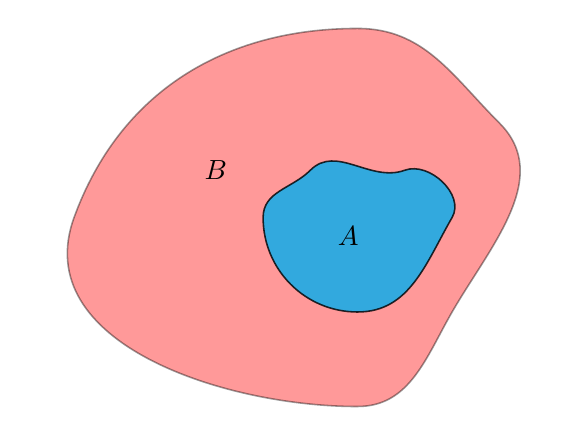
\begin{tikzpicture}[line width=0.2mm, scale=1.2]

    % Coordinates for the bigger blob.
    \coordinate (P1) at ( 0.0, -2.0);
    \coordinate (P2) at ( 1.0, -1.0);
    \coordinate (P3) at ( 1.5,  1.0);
    \coordinate (P4) at ( 0.0,  2.0);
    \coordinate (P5) at (-3.0,  0.0);

    % Coordinates for the inner blob.
    \coordinate (Q1) at ( 0.0, -1.0);
    \coordinate (Q2) at ( 1.0,  0.0);
    \coordinate (Q3) at ( 0.5,  0.5);
    \coordinate (Q4) at (-0.5,  0.5);
    \coordinate (Q5) at (-1.0,  0.0);

    % Coordindates to label things.
    \coordinate (A) at (-0.1, -0.2);
    \coordinate (B) at (-1.5,  0.5);

    % Draw the bigger blob.
    \draw[fill=red, opacity=0.4] (P1) to [out=0,    in=-120] (P2)
                                      to [out=60,   in=-45]  (P3)
                                      to [out=135,  in=0]    (P4)
                                      to [out=-180, in=70]   (P5)
                                      to [out=-110, in=-180] cycle;

    % Draw the inner blob.
    \draw[fill=cyan, opacity=0.8] (Q1) to [out=0,    in=-120]  (Q2)
                                       to [out=60,   in=20]    (Q3)
                                       to [out=-160, in=45]    (Q4)
                                       to [out=-135, in=90]    (Q5)
                                       to [out=-90,  in=180]   cycle;

    % Labels for the two blobs.
    \node at (A) {$A$};
    \node at (B) {$B$};
\end{tikzpicture}

            \caption{Visualizing Subsets as Blobs}
            \label{fig:Subset_Blobs}
        \end{figure}
        \begin{example}
            Consider the set of natural numbers $\mathbb{N}$ and the set of
            integers $\mathbb{Z}$ (loosely defined in
            Eqn.~\ref{eqn:Natural_Numbers_Ellipses} and
            Eqn.~\ref{eqn:Integers_Ellipses}, respectively). It can be seen that
            every natural number is also an integer, and thus we have:
            \begin{equation}
                \mathbb{N}\subseteq\mathbb{Z}
            \end{equation}
            Letting \gls{mathbbQ} denote the rational
            numbers\index{Rational Numbers} $p/q$, where $p,q\in\mathbb{Z}$ and
            $q$ is non-zero, we can see that $\mathbb{Q}$ contains $\mathbb{Z}$
            as a subset. That is, setting $q=1$ and allowing $p$ to vary over
            $\mathbb{Z}$ gives us every integer. Thus:
            \begin{equation}
                \mathbb{Z}\subseteq\mathbb{Q}
            \end{equation}
            We can continue with the real numbers (\gls{mathbbR}) and the
            complex numbers (\gls{mathbbC}) as well, creating a chain of
            subsets:
            \begin{equation}
                \mathbb{N}\subseteq\mathbb{Z}\subseteq\mathbb{Q}
                \subseteq\mathbb{R}\subseteq\mathbb{C}
            \end{equation}
        \end{example}
        \begin{example}
            Let $\mathbb{Z}_{n}$ be the set of all integers $k\in\mathbb{N}$
            such that $k<n$. If $m,n\in\mathbb{N}$ and $m<n$ we see that:
            \begin{equation}
                \mathbb{Z}_{m}\subseteq\mathbb{Z}_{n}
            \end{equation}
            This is because $\mathbb{Z}_{m}$ is the set of all $k\in\mathbb{N}$
            such that $k<m$. But since $\mathbb{Z}_{n}$ is the set of all
            $k\in\mathbb{N}$ such that $k<n$, and since $m<n$, if
            $k\in\mathbb{Z}_{m}$ then $k<m$, and thus $k<n$, which implies that
            $k\in\mathbb{Z}_{n}$.
        \end{example}
        It is important to note the distinction between the symbols for
        containment (\gls{containmentsymb}) for for subset\index{Set!Subset}
        (\gls{subseteq}). The symbol $\in$ is used to denote that some object
        $x$ is an \textit{element}\index{Set!Element of} of some set. That is,
        $x\in{A}$ indicates that $x$ is an element of $A$. This does not
        necessarily imply $x\subseteq{A}$, but this \textit{does} imply that
        $\{x\}\subseteq{A}$. That is, if $x\in{A}$, then the set that contains
        only $x$ is a subset of $A$. Moreover, the notions are not mutually
        exclusive. It is possible for $A$ to be a set such that $x\in{A}$ and
        $x\subseteq{A}$. For let $A=\{\emptyset\}$. For any set $A$ it is true
        that $\emptyset\subseteq{A}$ (see Thm.~\ref{thm:Emptyset_Is_Subset}).
        But from how $A$ is defined, we have that $\emptyset\in{A}$. Thus it is
        true that both $\emptyset\in{A}$ and $\emptyset\subseteq{A}$.
        \begin{fexample}{Elementary Examples of Subsets}
                        {Elementary_Examples_of_Subsets}
            Let $A$ and $B$ be the sets defined by:
            \par
            \begin{subequations}
                \begin{minipage}[b]{0.49\textwidth}
                    \centering
                    \begin{equation}
                        A=\big\{\,a,\,b,\,c\,\big\}
                    \end{equation}
                \end{minipage}
                \hfill
                \begin{minipage}[b]{0.49\textwidth}
                    \centering
                    \begin{equation}
                        B=\big\{\,a,\,b,\,c,\,d\,\big\}
                    \end{equation}
                \end{minipage}
            \end{subequations}
            \par\vspace{2.5ex}
            where we assume that $a$, $b$, $c$, and $d$ are distinct objects.
            From the definition of subsets (Def.~\ref{def:Subsets}):
            \par
            \begin{subequations}
                \begin{minipage}[b]{0.49\textwidth}
                    \centering
                    \begin{equation}
                        A\subseteq{B}
                    \end{equation}
                \end{minipage}
                \hfill
                \begin{minipage}[b]{0.49\textwidth}
                    \centering
                    \begin{equation}
                        B\nsubseteq{A}
                    \end{equation}
                \end{minipage}
            \end{subequations}
            \par\vspace{2.5ex}
            This is true since from the definition of $A$ and $B$, every element
            of $A$ is also an element of $B$. The converse of this is not true
            since there is an element of $B$ that is not an element of $A$
            (namely, the element $d$). That is, $d\in{B}$ but $d\notin{A}$ and
            therefore $B\nsubseteq{A}$.
        \end{fexample}
        The example shown in Ex.~\ref{ex:Elementary_Examples_of_Subsets} hints
        at how we can redefine equality of sets. We see that $A\subseteq{B}$,
        but $B\nsubseteq{A}$. If we have two sets $A$ and $B$ such that
        $A\subseteq{B}$ and $B\subseteq{A}$, then it would be impossible to
        discern between the two. This gives us our new definition of equality.
        We now prove this equivalence with the axiom of extensionality%
        \index{Axiom!of Extensionality} (Ax.~\ref{ax:Axiom_of_Extensionality}).
        \begin{theorem}
            \label{thm:Equivalent_Def_of_Equality}%
            If $A$ and $B$ are sets, then $A=B$ if and only if $A\subseteq{B}$
            and $B\subseteq{A}$.
        \end{theorem}
        \begin{proof}
            By the axiom of extensionality
            (Ax.~\ref{ax:Axiom_of_Extensionality}), $A=B$ if and only if for
            all $x$ it is true that $x\in{A}$ if and only if $x\in{B}$. But then
            $x\in{A}$ implies that $x\in{B}$, and thus $A\subseteq{B}$
            (Def.~\ref{def:Subsets}). But also $x\in{B}$ implies $x\in{A}$, and
            therefore $B\subseteq{A}$. Therefore if $A=B$, then $A\subseteq{B}$
            and $B\subseteq{A}$. Now if $A\subseteq{B}$ and $B\subseteq{A}$,
            then for all $x\in{A}$ it is true that $x\in{B}$ and for all
            $x\in{B}$ it is true that $x\in{A}$ (Def.~\ref{def:Subsets}), and
            therefore $x\in{A}$ if and only if $x\in{B}$. Thus if
            $A\subseteq{B}$ and $B\subseteq{A}$, then $A=B$. But it was just
            proved that if $A=B$, then $A\subseteq{B}$ and $B\subseteq{A}$.
            Therefore $A=B$ if and only if $A\subseteq{B}$ and $B\subseteq{A}$.
        \end{proof}
        With this, we can redefine the notion of
        \textit{equal sets}\index{Set!Equal Sets}.
        \begin{fdefinition}{Equal Sets}{Equal_Sets}
            \Glspl{equal set} are \glspl{set} $A$ and $B$, denoted
            \glslink{equalsymb}{$A=B$}, such that $A\subseteq{B}$ and
            $B\subseteq{A}$.\index{Set!Equality}
            \begin{equation*}
                \forall_{A}\forall_{B}\Big((A=B)\Longleftrightarrow
                \big((A\subseteq{B})\land(B\subseteq{A})\big)\Big)
            \end{equation*}
        \end{fdefinition}
        Def.~\ref{def:Equal_Sets} is justified by
        Thm.~\ref{thm:Equivalent_Def_of_Equality}, and thus there is no
        contradiction with the axiom of extensionality
        (Ax.~\ref{ax:Axiom_of_Extensionality}). If $A$ and $B$ are not equal, we
        write $A\ne{B}$. 
        \begin{lexample}{More Examples of Subsets}{More_Examples_of_Subsets}
            Using the notation from Ex.~\ref{ex:Using_Element_Notation}, for all
            $n\in\mathbb{N}$ we have:
            \begin{equation}
                \mathbb{Z}_{n}\subseteq\mathbb{N}
            \end{equation}
            Let's define \gls{mathbbNe} and \gls{mathbbNo} to be the sets of
            even\index{Natural Numbers!Even} and odd\index{Natural Numbers!Odd}
            non-negative integers, respectively:
            \par
            \begin{subequations}
                \begin{minipage}[b]{0.49\textwidth}
                    \centering
                    \begin{equation}
                        \label{eqn:Even_Pos_Ints_Ellipses}%
                        \mathbb{N}_{e}=\big\{\,0,\,2,\,4,\,6,\,8,\,\dots\,\big\}
                    \end{equation}
                \end{minipage}
                \hfill
                \begin{minipage}[b]{0.49\textwidth}
                    \centering
                    \begin{equation}
                        \label{eqn:Odd_Pos_Ints_Ellipses}%
                        \mathbb{N}_{o}=\big\{\,1,\,3,\,5,\,7,\,9,\,\dots\,\big\}
                    \end{equation}
                \end{minipage}
            \end{subequations}
            \par\vspace{2.5ex}
            From this we see the following two expressions are true:
            \par
            \begin{subequations}
                \begin{minipage}[b]{0.49\textwidth}
                    \centering
                    \begin{equation}
                        \mathbb{N}_{o}\subseteq\mathbb{N}
                    \end{equation}
                \end{minipage}
                \hfill
                \begin{minipage}[b]{0.49\textwidth}
                    \centering
                    \begin{equation}
                        \mathbb{N}_{e}=\mathbb{N}
                    \end{equation}
                \end{minipage}
            \end{subequations}
            \par\vspace{2.5ex}
            Moreover we see that $\mathbb{N}_{o}$ and $\mathbb{N}_{e}$ have no
            elements in common. That is, they are \textit{disjoint}%
            \index{Set!Disjoint Sets}. From this, we can write:
            \par
            \begin{subequations}
                \begin{minipage}[b]{0.49\textwidth}
                    \centering
                    \begin{equation}
                        \mathbb{N}_{o}\nsubseteq\mathbb{N}_{e}
                    \end{equation}
                \end{minipage}
                \hfill
                \begin{minipage}[b]{0.49\textwidth}
                    \centering
                    \begin{equation}
                        \mathbb{N}_{e}\nsubseteq\mathbb{N}_{o}
                    \end{equation}
                \end{minipage}
            \end{subequations}
            \par\vspace{2.5ex}
            We can also think of trivial examples:
            \par
            \begin{subequations}
                \begin{minipage}[b]{0.49\textwidth}
                    \centering
                    \begin{equation}
                        \mathbb{Z}_{3}\subseteq\mathbb{Z}_{4}
                    \end{equation}
                \end{minipage}
                \hfill
                \begin{minipage}[b]{0.49\textwidth}
                    \centering
                    \begin{equation}
                        \mathbb{Z}_{4}\nsubseteq\mathbb{Z}_{3}
                    \end{equation}
                \end{minipage}
            \end{subequations}
            \par\vspace{2.5ex}
            This is because every element of $\mathbb{Z}_{3}$ is contained in
            $\mathbb{Z}_{4}$, but $3\in\mathbb{Z}_{4}$ and
            $3\notin\mathbb{Z}_{3}$.
        \end{lexample}
        It may seem like bad notation to write $3\notin\mathbb{Z}_{3}$, but
        since we want $\mathbb{Z}_{n}$ to have $n$ elements, and since we
        started counting at zero, we have that $n\notin\mathbb{Z}_{n}$ for all
        $n\in\mathbb{N}$. Such counting schemes are common in computer science,
        but there's disagreement in mathematics as to whether $0\in\mathbb{N}$
        or not. We will use the
        \textit{axiom of infinity}\index{Axiom!of Infinity} to prove the
        existence of $\mathbb{N}$, and in doing so it will be natural to define
        $\mathbb{N}$ as a set that contains $0$.
        \par\hfill\par
        While Def.~\ref{def:Equal_Sets} is indeed equivalent to the axiom of
        extensionality, this definition creates a few problems. As discussed
        previously, sets have no notion of order and cannot account for
        repetition. For let $A$, $B$, and $C$ be the sets defined by:
        \par
        \begin{subequations}
            \begin{minipage}[b]{0.31\textwidth}
                \centering
                \begin{equation}
                    A=\big\{\,a,\,b\,\big\}
                \end{equation}
            \end{minipage}
            \hfill
            \begin{minipage}[b]{0.36\textwidth}
                \centering
                \begin{equation}
                    B=\big\{\,a,\,a,\,b\,\big\}
                \end{equation}
            \end{minipage}
            \hfill
            \begin{minipage}[b]{0.31\textwidth}
                \centering
                \begin{equation}
                    C=\big\{\,b,\,a\,\big\}
                \end{equation}
            \end{minipage}
        \end{subequations}
        \par\vspace{2.5ex}
        All three of these sets are equal by both the definition of equality
        (Def.~\ref{def:Equal_Sets})\index{Set!Equal Sets} and the axiom of
        extensionality\index{Axiom!of Extensionality}. It seems clear that
        $A\subseteq{B}$, but it is also true that $B\subseteq{A}$. This is
        because $B$ contains only the elements $a$ and $b$. While $a$ is
        included twice, repetition cannot be accounted for and $B$ is entirely
        determined by $a$ and $b$. But $A$ also contains $a$ and $b$, and
        therefore $B\subseteq{A}$. By the definition of equality
        (Def.~\ref{def:Equal_Sets}), we have that $A=B$. In a similar manner,
        $A=C$. From the definition of subsets, for any set $A$ we see that
        $A\subseteq{A}$ (see Thm.~\ref{thm:Reflexivity_of_Inclusion}). It would
        be nice to distinguish between subsets that aren't the entire set
        itself. These are called proper subsets\index{Set!Subset!Proper}, and
        we can define them in terms of equality.
        \begin{fdefinition}{Proper Subsets}{Proper_Subsets}
            A \gls{proper subset} of a \gls{set} $B$ is a set $A$ such that
            $A\subseteq{B}$ and $A\ne{B}$. We write
            \glslink{subsetneq}{$A\subsetneq{B}$} to denote that $A$ is a proper
            subset of $B$.\index{Set!Subset!Proper}
            \begin{equation*}
                \forall_{A}\forall_{B}(A\subsetneq{B})
                \Longleftrightarrow\Big((A\subseteq{B})\land(A\ne{B})\Big)
            \end{equation*}
        \end{fdefinition}
        The symbols \gls{subseteq} and \gls{subsetneq} are analogous to the
        notations of inequalities that one finds in calculus: \gls{leq} and
        \gls{lessthan}. In many texts, the two symbols $\subseteq$ and $\subset$
        are taken to be identical, which may cause confusion. In an attempt to
        reduce confusion, $\subseteq$ will denote any subset, $\subsetneq$
        denotes a proper subset, and the symbol $\subset$ will be avoided.
        \begin{lexample}{Proper Subsets}{Proper_Subsets}
            Let $A$ and $B$ be sets defined as follows:
            \par
            \begin{subequations}
                \begin{minipage}[b]{0.49\textwidth}
                    \centering
                    \begin{equation}
                        A=\big\{\,a,\,b,\,c\,\big\}
                    \end{equation}
                \end{minipage}
                \hfill
                \begin{minipage}[b]{0.49\textwidth}
                    \centering
                    \begin{equation}
                        B=\big\{\,a,\,b,\,c,\,d\,\big\}
                    \end{equation}
                \end{minipage}
            \end{subequations}
            \par\vspace{2.5ex}
            Then $A\subseteq{B}$, since every element of $A$ is an element of
            $B$, but $B\nsubseteq{A}$ since $d\in{B}$ and $d\notin{A}$.
            Therefore $A\ne{B}$, and thus $A$ is a proper subset of $B$. We can
            denote this by writing $A\subsetneq{B}$.
        \end{lexample}
        Proper subsets are subsets that are missing at least one element
        (see Thm.~\ref{thm:Prop_Subset_Not_Equal}). Returning to our claim that
        $\emptyset\subseteq{A}$ for any set $A$, for any non-empty set $A$ we
        have that $\emptyset\subsetneq{A}$. This is because for non-empty sets
        there is at least one $x$ such that $x\in{A}$
        (Def.~\ref{def:Non_Empty_Set}), whereas for all $x$ it is true that
        $x\notin\emptyset$. Thus equality cannot occur, and the empty set must
        be a proper subset. It is also true that the empty set contains no
        proper subsets. The only subset of $\emptyset$ is itself.
        \begin{example}
            Returning to more concrete examples, $\mathbb{N}$ is a proper subset
            of $\mathbb{Z}$. To see this, note that $\minus{1}\in\mathbb{Z}$ but
            $\minus{1}\notin\mathbb{N}$. Indeed, none of the negative integers
            are natural numbers, but they are integers. We can write this by:
            \begin{equation}
                \mathbb{N}\subsetneq\mathbb{Z}
            \end{equation}
            Similarly, $\mathbb{Q}$ contains numbers that are not integers,
            for example $1/2$. Thus, $\mathbb{Z}$ is also a proper subset of
            $\mathbb{Q}$. Lastly, since $\sqrt{2}$ is not a rational number, the
            set of rational numbers must then be a proper subset of the set of
            real numbers.
        \end{example}
        We now introduce the \textit{axiom schema of specification}.
        \begin{faxiom}{Axiom Schema of Specification}
                      {Axiom_Schema_of_Specification}
            If $A$ is a set and if $P$ is a proposition, then there exists a set
            $B$ such that $x\in{B}$ if and only if $x\in{A}$ and $P(x)$ is true.
            We can write this as:\index{Axiom!Schema of Specification}
            \index{Proposition}
            \begin{equation*}
                B=\big\{\,x\in{A}\;|\;P(x)\,\big\}
            \end{equation*}
            Using our formal language, we have:
            \begin{equation*}
                \forall_{A}\forall_{P}\exists_{B}:
                \forall_{x}\Big((x\in{B})\Leftrightarrow
                \big((x\in{A})\land{P}(x)\big)\Big)
            \end{equation*}
        \end{faxiom}
        Ax.~\ref{ax:Axiom_Schema_of_Specification} is different from the
        inconsistent axiom of unrestricted comprehension%
        \index{Axiom!of Unrestricted Comprehension} in that we can only speak of
        elements that are already defined and contained in some other set. That
        is, this new axiom does not allow us to talk about the
        \textit{set of all sets}\index{Set!of All Sets}, and so we have avoided
        the crux of Russell's paradox.\index{Russell's Paradox}
        \par\hfill\par
        This allows us to use the Set-Builder\index{Set-Builder Notation} method
        of constructing sets. We described the natural numbers \gls{mathbbN} and
        integers \gls{mathbbZ} (From the German \textit{Zahl}) using
        Eqns.~\ref{eqn:Natural_Numbers_Ellipses} and
        \ref{eqn:Integers_Ellipses}, respectively. It would be more difficult
        (but not impossible) to describe the set of rational numbers%
        \index{Rational Numbers} in such a way. Instead, we use set-builder
        notation if it is known that \gls{mathbbQ} is contained in some larger
        set \gls{mathbbR} (the \textit{real} numbers)\index{Real Numbers}.
        \begin{equation}
            \mathbb{Q}=\Big\{\;\frac{p}{q}\in\mathbb{R}\;\big|\;
                                p,\,q\in\mathbb{Z}\textrm{ and }q\ne{0}\;\Big\}
        \end{equation}
        That is, the rational numbers are the set of all real numbers which can
        be written as the ratios of integers with non-zero denominator. The
        Axiom Schema of Specification states that this is is a valid method of
        describing sets. It is also known as the axiom of separation%
        \index{Axiom!of Separation}.
        \begin{example}
            We can describe the sets $\mathbb{Z}$, $\mathbb{N}$,
            $\mathbb{N}_{e}$, and $\mathbb{N}_{o}$ using set-builder notation if
            we assume these belong to some larger set $\mathbb{R}$. We define
            $\mathbb{Z}$ by:
            \index{Natural Numbers}\index{Natural Numbers!Even}%
            \index{Natural Numbers!Odd}\index{Integers}
            \begin{equation}
                \mathbb{Z}=
                \big\{\,n\in\mathbb{R}\;|\;n\textrm{ is an integer}\,\big\}
            \end{equation}
            From here we can define $\mathbb{N}$ by:
            \begin{equation}
                \mathbb{N}=\{\,n\in\mathbb{Z}\;|\;n\geq{0}\,\}
            \end{equation}
            Furthermore, $\mathbb{N}_{e}$ and $\mathbb{N}_{0}$ can be described
            as follows:
            \par
            \begin{subequations}
                \begin{minipage}[b]{0.495\textwidth}
                    \centering
                    \begin{equation}
                        \label{eqn:Even_Pos_Ints_Set_Builder}%
                        \mathbb{N}_{e}=
                        \big\{n\in\mathbb{N}\;|\;n\textrm{ is even}\big\}
                    \end{equation}
                \end{minipage}
                \hfill
                \begin{minipage}[b]{0.495\textwidth}
                    \centering
                    \begin{equation}
                        \label{eqn:Odd_Pos_Ints_Set_Builder}%
                        \mathbb{N}_{o}=
                        \big\{n\in\mathbb{N}\;|\;n\textrm{ is odd}\big\}
                    \end{equation}
                \end{minipage}
            \end{subequations}
            \par\vspace{2.5ex}
            Such notation is justified by the axiom schema of specification%
            \index{Axiom!Schema of Specification}.
        \end{example}
        We are not adopting these definitions since they lack rigor. These
        examples build intuition behind the notation and the axioms, but we will
        develop arithmetic axiomatically using the \textit{axiom of infinity}%
        \index{Axiom!of Infinity}.
        \begin{example}
            Concrete examples of set builder notation can be made if we examine
            propositions that lead to finite sets. Consider the set $A$ defined
            by:
            \begin{equation}
                S=\{\,n\in\mathbb{N}\;|\;\textit{There exists }k\in\mathbb{N}
                    \textit{ such that }k<5\textit{ and }n=7k-3\,\}
            \end{equation}
            It may be easier if we rewrite this as follows:
            \begin{equation}
                S=\{\,7k-3\;|\;k\in\mathbb{N}\textrm{ and }k<5\}
            \end{equation}
            So we just need to loop through this equatio from $k=0$ to $k=4$.
            We obtain:
            \begin{equation}
                S=\{\,\minus{3},\,4,\,11,\,18,\,24\,\}
            \end{equation}
        \end{example}
    \subsection{Ordered Pairs and Unions}
        We now wish to solve the issue previously raised that sets do
        not have order. We'll develop a new object, called ordered pairs%
        \index{Ordered Pair}, that can distinguish such things. The definition
        we'll adopt is due to Kuratowski\index{Kuratowski, Kazimierz} and
        defines \gls{orderedpairsymb} as follows:
        \begin{equation}
            (a,\,b)=\big\{\,\{\,a\,\},\,\{\,a,\,b\,\}\,\big\}
        \end{equation}
        We now prove such a set exists within the framework of \gls{ZFC}.
        \begin{faxiom}{Axiom of Pairing}{Axiom_of_Pairing}
            If $A$ and $B$ are sets, then there exists a set $\mathcal{C}$
            such that $A\in\mathcal{C}$ and $B\in\mathcal{C}$.
            \index{Axiom!of Pairing}
            \begin{equation*}
                \forall_{A}\forall_{B}\exists_{\mathcal{C}}:
                \Big((A\in\mathcal{C})\land(B\in\mathcal{C})\Big)
            \end{equation*}
        \end{faxiom}
        The set hypothesized to exist in this axiom may be very large, we have
        no way of knowing. What we want from this is a set that contains two
        elements $A$ and $B$, and only those elements. We obtain this by
        combining pairing with specification.
        \begin{theorem}
            \label{thm:Existence_of_Set_Built_from_Two_Sets}%
            If $A$ and $B$ are sets, then there exists a set $D$ such that
            for all $x$ it is true that $x\in{D}$ if and only if $x=A$ or
            $x=B$. That is:
            \begin{equation}
                D=\{\,A,\,B\,\}
            \end{equation}
        \end{theorem}
        \begin{proof}
            By the axiom of pairing (Ax.~\ref{ax:Axiom_of_Pairing}) there
            exists a set $\mathcal{C}$ such that $A\in\mathcal{C}$ and
            $B\in\mathcal{C}$. Let $P$ be the proposition
            \textit{true if} $x=A$ \textit{or} $x=B$, \textit{false otherwise}.
            By the axiom schema of specification
            (Ax.~\ref{ax:Axiom_Schema_of_Specification}), there is a set
            $D$ such that:
            \begin{equation}
                D=\{\,x\in\mathcal{C}\;|\;P(x)\,\}
            \end{equation}
            That is, $x\in{D}$ if and only if $x\in\mathcal{C}$ and $P(x)$ is
            true. But then $x\in{D}$ if and only if $x\in\mathcal{C}$ and $x=A$
            or $x\in\mathcal{C}$ and $x=B$. But $A\in\mathcal{C}$ and
            $B\in\mathcal{C}$, and thus $P(x)$ implies $x\in\mathcal{C}$. Thus,
            $x\in{D}$ if and only if $P(x)$ is true. That is, $x\in{D}$ if and
            only if $x=A$ or $x=B$.
        \end{proof}
        By the axiom of extensionality\index{Axiom!of Extensionality}
        (Ax.~\ref{ax:Axiom_of_Extensionality}), the set hypothesized in
        Thm.~\ref{thm:Existence_of_Set_Built_from_Two_Sets} is unique, and thus
        there is no trouble in \textit{defining} the symbol $\{A,B\}$ to be the
        unique set that contains the elements $A$ and $B$ and only those
        elements. That is, we develop the new notation:
        \begin{fnotation}{Finite Set Notation}{Finite_Set_Notation}
            If $A$ and $B$ are sets, then $\{A,B\}$ is the unique set such that
            for all $x$, $x\in\{A,B\}$ if and only if $x=A$ or $x=B$.
            \index{Set!Finite}
            \begin{equation*}
                \forall_{x}\Big(\big(x\in\{A,B\}\big)
                \Longleftrightarrow\big((x=A)\lor(x=B)\big)\Big)
            \end{equation*}
        \end{fnotation}
        \begin{theorem}
            \label{thm:Existence_of_Set_Containing_Set}%
            If $A$ is a set, then there is a set $B$ such that $x\in{B}$ if
            and only if $x=A$. That is, there exists a set $B$ such that:
            \begin{equation}
                B=\{\,A\,\}
            \end{equation}
        \end{theorem}
        \begin{proof}
            For since $A$ is a set, by
            Thm.~\ref{thm:Existence_of_Set_Built_from_Two_Sets} there exists
            a set $B=\{A,\,A\}$. But then $x\in{B}$ if and only if $x=A$.
        \end{proof}
        We can apply Not.~\ref{not:Finite_Set_Notation} to a single set $A$ and
        similarly define what the notation $\{A\}$ means. With this, we can now
        prove the existence of ordered pairs.
        \begin{ltheorem}{Existence of Ordered Pairs}{Existence_of_Ordered_Pairs}
            If $A$ and $B$ are sets, then there is a set $(A,\,B)$ such that
            for all $x$ it is true that $x\in(A,\,B)$ if only if $x=\{A\}$
            or $x=\{A,B\}$.\index{Ordered Pair}
        \end{ltheorem}
        \begin{proof}
            For by Thm.~\ref{thm:Existence_of_Set_Containing_Set}, there is
            a set $\{A\}$ such that $x\in\{A\}$ if and only if $x=A$.
            But by Thm.~\ref{thm:Existence_of_Set_Built_from_Two_Sets}, there
            is a set $\{A,\,B\}$ such that $x\in\{A,\,B\}$ and if only
            if $x=A$ or $x=B$. But again by
            Thm.~\ref{thm:Existence_of_Set_Built_from_Two_Sets}, since
            $\{A\}$ and $\{A,\,B\}$ are sets, there is a set $(A,\,B)$ such
            that $x\in(A,\,B)$ if and only if $x=\{A\}$ or $x=\{A,\,B\}$.
        \end{proof}
        \begin{fdefinition}{Ordered Pairs}{Ordered_Pairs}
            The \gls{ordered pair} of a \gls{set} $x$ with respect to a set
            $y$ is the set:\index{Ordered Pair}
            \begin{equation*}
                (x,\,y)=\big\{\,\{\,x\,\},\,\{\,x,\,y\,\}\,\big\}
            \end{equation*}
            Using our formal language:
            \begin{equation*}
                \forall_{x}\forall_{y}\forall_{z}\Big(
                    \big(z\in(x,y)\big)\Longleftrightarrow
                    \big((z=\{x\})\lor(z=\{x,y\})\big)
                \Big)
            \end{equation*}
        \end{fdefinition}
        Thm.~\ref{thm:Existence_of_Ordered_Pairs} asserts the existence of
        ordered pairs\index{Ordered Pair}, as defined by Kuratowski%.
        \index{Kuratowski, Kazimierz}, and allows us to present
        Def.~\ref{def:Ordered_Pairs} in a way that is consistent with ZFC.
        Kuratowski first put forward this definition in 1921 and it does
        precisely what we want it to do and orders elements. That is, if $x$ and
        $y$ are distinct, then $(x,\,y)\ne(y,\,x)$. The caveat with this
        definition is the following reduction:
        \begin{equation}
            (x,\,x)
            =\big\{\,\{\,x\,\},\,\{\,x,\,x\,\}\,\big\}
            =\big\{\,\{\,x\,\},\{\,x\,\}\,\big\}
            =\big\{\,\{\,x\,\}\,\big\}
        \end{equation}
        Prior to Kuratowski there existed a definition due to Norbert Wiener%
        \index{Wiener, Norbert}, put forward in 1914. His definition grew out of
        Bertrand Russell's\index{Russell, Bertrand} Type
        Theory\index{Type Theory} which was an attempt to rid set theory of the
        paradoxes he discovered. Wiener writes:
        \begin{equation}
            (x,\,y)_{W}=\Big\{\,\big\{\,\{\,x\,\},\,\emptyset\,\big\},\,
                                \big\{\,\{\,y\,\}\,\big\}\Big\}
        \end{equation}
        Returning to Kuratowski's definition (Def.~\ref{def:Ordered_Pairs}),
        consider the ordered pair $(1,\,2)$, where we take for granted that
        $1\ne{2}$. We have:
        \begin{equation}
            (1,\,2)=\big\{\,\{\,1\,\},\,\{\,1,\,2\,\}\,\big\}
        \end{equation}
        Swapping and computing $(2,\,1)$, we obtain:
        \begin{equation}
            (2,\,1)=\big\{\,\{\,2\,\},\,\{\,2,\,1\,\}\,\big\}
        \end{equation}
        We know that sets cannot distinguish order, so
        $\{\,1,\,2\,\}=\{\,2,\,1\,\}$. Thus:
        \par
        \begin{subequations}
            \begin{minipage}[b]{0.49\textwidth}
                \centering
                \begin{equation}
                    (1,\,2)=\big\{\,\{\,1\,\},\,\{\,1,\,2\,\}\,\big\}
                \end{equation}
            \end{minipage}
            \hfill
            \begin{minipage}[b]{0.49\textwidth}
                \centering
                \begin{equation}
                    (2,\,1)=\big\{\,\{\,2\,\},\,\{\,1,\,2\,\}\,\big\}
                \end{equation}
            \end{minipage}
        \end{subequations}
        \par\vspace{2.5ex}
        Combining these equations, we now have that:
        \begin{equation}
            (1,\,2)\ne(2,\,1)
        \end{equation}
        To see this, note that both sets contain the element $\{1,\,2\}$, but
        $\{1\}$ is an element of $(1,\,2)$ and not an element of $(2,\,1)$,
        and thus $(1,\,2)\nsubseteq(2,\,1)$. Similarly, $\{2\}$ is an element
        of $(2,\,1)$ but not an element of $(1,\,2)$, and therefore
        $(2,\,1)\nsubseteq(1,\,2)$. From the definition of equality
        (Def.~\ref{def:Equal_Sets}), we have that these sets are not equal.
        \par\hfill\par
        There's is an unfortunate doubling of notation that occurs in
        mathematics, and $(a,b)$ has two common meanings. The first meaning is
        the ordered pair which we've just defined, and the second is the
        \textit{open interval}\index{Interval!Open} defined in the context of a
        \textit{partially ordered set}\index{Partially Ordered Set}.
        The most common example is when discussing the real numbers
        $\mathbb{R}$, $(a,b)$ denotes the set of all real numbers $x$ such that
        $a<x$ and $x<b$. Hopefully it will be clear what the notation means when
        a theorem or example is being presented, but we will be explicit when
        ambiguity can arise.
        \par\hfill\par
        The natural thing from here is to construct the
        \textit{Cartesian Product}\index{Cartesian Product} of two sets. This is
        the set of all ordered pairs\index{Ordered Pair} $(a,\,b)$ where $a$
        belongs to some set $A$ and $b$ belongs to another set $B$. To prove
        such a set exists requires two more axioms.
        \newpage
        \begin{faxiom}{Axiom of Union}{Axiom_of_Union}
            If $\mathcal{O}$ is a set, then there exists a set $\mathcal{F}$
            such that, for all $A$ such that $A\in\mathcal{O}$ and for all
            $x$ such that $x\in{A}$, it is true that $x\in\mathcal{F}$.%
            \index{Axiom!of Union}
            \begin{equation*}
                \forall_{\mathcal{O}}\exists_{\mathcal{F}}:\forall_{x}\Big(
                \big(\exists_{A\in\mathcal{O}}:x\in{A}\big)
                \Rightarrow{x}\in\mathcal{F}\Big)
            \end{equation*}
        \end{faxiom}
        This states that, given a collection of sets $\mathcal{O}$, there exists
        a larger set which contains the elements of the constituent sets of
        $\mathcal{O}$. Similar to the axiom of pairing, $\mathcal{F}$ may be
        much larger than desired and we must invoke the axiom schema of
        specification to arrive at the \textit{union} over a collection.
        \begin{ltheorem}{Existence of the Union of Sets}{Existence_of_Unions}
            If $\mathcal{O}$ is a set, then there exists a set \gls{unionO} such
            that for all $x$ it is true that $x\in\bigcup\mathcal{O}$ if and
            only if there is a set $A\in\mathcal{O}$ such that $x\in{A}$.
        \end{ltheorem}
        \begin{proof}
            For by the axiom of union (Ax.~\ref{ax:Axiom_of_Union}), there
            exists a set $\mathcal{F}$ such that for all $A\in\mathcal{O}$
            and for all $x\in{A}$ it is true that $x\in\mathcal{F}$. Let
            $P$ be the proposition \textit{true if there exists a set}
            $A\in\mathcal{O}$ \textit{such that} $x\in{A}$,
            \textit{false otherwise}. Then, by the axiom schema of specification
            (Ax.~\ref{ax:Axiom_Schema_of_Specification}) there exists a set
            $\bigcup\mathcal{O}$ such that:
            \begin{equation}
                \bigcup\mathcal{O}=\big\{\,x\in\mathcal{F}\;|\;P(x)\,\big\}
            \end{equation}
            But then $x\in\bigcup\mathcal{O}$ if and only if $x\in\mathcal{F}$
            and $P(x)$ is true. But if $P(x)$ is true, then $x\in\mathcal{F}$,
            and thus $x\in\bigcup\mathcal{O}$ if and only if there is a set
            $A\in\mathcal{O}$ such that $x\in{A}$.
        \end{proof}
        One question that arises is
        \textit{what happens if our collection is empty}? That is, if
        $\mathcal{O}=\emptyset$, is there any meaning behind the equation:
        \begin{equation}
            \mathcal{F}=\bigcup\emptyset
        \end{equation}
        There is, and $\mathcal{F}$ will be the empty set. That is,
        $\mathcal{F}=\emptyset$. This is true in a vacuous sense and can be
        proved via contradiction with the law of the excluded middle.
        We define the set $\mathcal{F}$ described in
        Thm.~\ref{thm:Existence_of_Unions} as the
        \textit{union}\index{Union!over a Collection}
        over the set $\mathcal{O}$. The set $\mathcal{O}$ is often called the
        index set\index{Index Set} for which we take the union over.
        \begin{fdefinition}{Union over a Set}{Union_over_a_Set}
            The \gls{union over a set} $\mathcal{O}$ is the set:
            \index{Set!Union}\index{Union!over a Collection}
            \begin{equation*}
                \bigcup_{\mathcal{U}\in\mathcal{O}}\mathcal{U}
                =\big\{\,x\;|\;\textrm{There exists a set }
                         \mathcal{U}\in\mathcal{O}\textrm{ such that }
                         x\in\mathcal{U}\big\}
            \end{equation*}
            Using our formal language:
            \begin{equation*}
                \forall_{\mathcal{O}}\forall_{x}\bigg(
                    \Big(x\in\bigcup_{\mathcal{U}\in\mathcal{O}}\mathcal{U}\Big)
                    \Longleftrightarrow\big(\exists_{\mathcal{U}\in\mathcal{O}}:
                    x\in\mathcal{U}\big)\bigg)
            \end{equation*}
        \end{fdefinition}
        There are two ways to write unions for arbitrary collections, and we
        will make use of both depending on scenario. The first manner we have
        already seen in Thm.~\ref{thm:Existence_of_Unions} where, given a
        collection $\mathcal{O}$, we wrote \gls{unionO} to denote the union over
        $\mathcal{O}$. The second is depicted in
        Def.~\ref{def:Union_over_a_Set}. That is, given $\mathcal{O}$ we write:
        \begin{equation}
            \bigcup\mathcal{O}=\bigcup_{\mathcal{U}\in\mathcal{O}}\mathcal{U}
        \end{equation}
        This alternative notation can be useful when we are using various
        indexing tricks to solve problems, or when combining unions with the
        various other set operations such as differences and intersections.
        \par\hfill\par
        The notion of union is very convenient if we already have a collection
        of sets defined, but it would be nice to form the union over two given
        sets without considering them as part of a larger collection. This can
        be done by combining the axiom of union\index{Axiom!of Union} with
        pairing\index{Axiom!of Pairing}.
        \begin{theorem}
            \label{thm:Union_of_Two_Sets_Exists}%
            If $A$ and $B$ are sets, then there exists a set \gls{AcupB} such
            that $x\in{A}\cup{B}$ if and only if either $x\in{A}$ or $x\in{B}$.
        \end{theorem}
        \begin{proof}
            For by Thm.~\ref{thm:Existence_of_Set_Built_from_Two_Sets} there
            exists a set $\mathcal{O}$ such that $y\in\mathcal{O}$ if and only
            if $y=A$ or $y=B$. That is, $\mathcal{O}=\{A,\,B\}$. But by
            Thm.~\ref{thm:Existence_of_Unions} there exists a set $A\cup{B}$
            such that $x\in{A}\cup{B}$ if and only if there exists a set
            $\mathcal{U}\in\mathcal{O}$ such that $x\in\mathcal{U}$. But then
            $x\in{A}\cup{B}$ if and only if either $x\in{A}$ or $x\in{B}$.
        \end{proof}
        This allows us to define our first \textit{operation} of two sets.
        \begin{fdefinition}{Union of Two Sets}{Union_of_Two_Sets}
            The \gls{union of two sets} $A$ and $B$ is the set \gls{AcupB}
            defined by:\index{Union!of Two Sets}
            \begin{equation*}
                A\cup{B}=\big\{\,x\;|\;x\in{A}\textrm{ or }x\in{B}\,\big\}
            \end{equation*}
            That is:
            \begin{equation*}
                \forall_{A}\forall_{B}\forall_{x}\Big(
                    \big(x\in{A}\cup{B}\big)
                    \Longleftrightarrow
                    \big((x\in{A})\lor(x\in{B})\big)
                \Big)
            \end{equation*}
        \end{fdefinition}
        In our definition of the union over a collection and the union of two
        sets we have slightly abused our set-builder
        notation\index{Set-Builder Notation}. The axiom schema of
        specification\index{Axiom!Schema of Specification} allows us to write a
        set as $A=\{\,x\in{B}\,|\,P(x)\,\}$ given some set $B$ that is already
        known to exists, and some proposition\index{Proposition} $P$. These two
        definitions (Defs.~\ref{def:Union_over_a_Set} and
        \ref{def:Union_of_Two_Sets}) are justified by the theorems we have
        proven, and so there is no contradiction.
        \begin{example}
            \label{ex:Union_of_Zm_and_Zn}%
            Again using the notation found in Eqn.~\ref{eqn:Z_n_Ellipses}, if we
            let $\mathbb{Z}_{n}$ denote the integers between $0$ and $n-1$, we
            have the following: If $m$ is less than $n$, then:
            \begin{equation}
                \mathbb{Z}_{m}\cup\mathbb{Z}_{n}=\mathbb{Z}_{n}
            \end{equation}
            This is because every element of $\mathbb{Z}_{m}$ is already
            and element of $\mathbb{Z}_{n}$, and thus taking the union adds
            nothing new to $\mathbb{Z}_{n}$, so the resulting set is
            $\mathbb{Z}_{m}$.
        \end{example}
        \begin{example}
            Denoting the even and odd non-negative integers by \gls{mathbbNe}
            and \gls{mathbbNo}, respectively, we see that:
            \index{Natural Numbers!Even}\index{Natural Numbers!Odd}
            \begin{equation}
                \mathbb{N}_{e}\cup\mathbb{N}_{o}=\mathbb{N}
            \end{equation}
            This is because every non-negative integer $n\in\mathbb{N}$ is
            either even or odd, and thus either $n\in\mathbb{N}_{e}$ or
            $n\in\mathbb{N}_{o}$. Taking the union therefore gives the entire
            set $\mathbb{N}$. The union does not add anything more than
            $\mathbb{N}$ since $\mathbb{N}_{e}\subseteq\mathbb{N}$ and
            $\mathbb{N}_{o}\subseteq\mathbb{N}$.
        \end{example}
        \begin{fexample}{Union of Two Sets}{Union_of_Two_Sets}
            Let $A$ and $B$ be the sets defined by:
            \par
            \begin{subequations}
                \begin{minipage}[b]{0.49\textwidth}
                    \centering
                    \begin{equation}
                        A=\{\,a,\,b,\,c\,\}
                    \end{equation}
                \end{minipage}
                \hfill
                \begin{minipage}[b]{0.49\textwidth}
                    \centering
                    \begin{equation}
                        B=\{\,c,\,1,\,2\,\}
                    \end{equation}
                \end{minipage}
            \end{subequations}
            \par\vspace{2.5ex}
            The union of $A$ and $B$ is the set that contains all of the
            elements of $A$ and all of the elements of $B$, and only such
            elements. That is:
            \begin{equation}
                A\cup{B}=\{\,a,\,b,\,c,\,1,\,2\,\}
            \end{equation}
            Even though $c\in{A}$ and $c\in{B}$, $c$ only appears once in the
            union. This is because sets cannot account for repetition, so
            including $c$ twice would be redundant.
        \end{fexample}
        The union of two sets can again be visualized by considering blobs
        in the plane. Let $A$ and $B$ be two circles that overlap somewhere in
        the middle. The union $A\cup{B}$ can then be represented by shading in
        the region covered by either $A$ or $B$
        (see Fig.~\ref{fig:Union_of_Two_Sets}). Such a drawing is called a
        \textit{Venn diagram}\index{Venn Diagram}.
        \begin{figure}[H]
            \centering
            \captionsetup{type=figure}
            %--------------------------------Dependencies----------------------------------%
%   tikz                                                                       %
%-------------------------------Main Document----------------------------------%
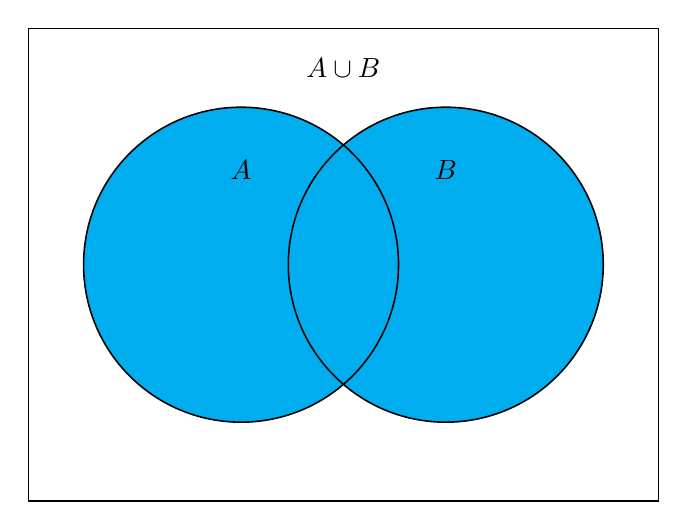
\begin{tikzpicture}[line width=0.2mm]

    % Coordinates for the centers of the circles.
    \coordinate (C1) at (-1.3, 0);
    \coordinate (C2) at ( 1.3, 0);

    % Coordinates for the labels.
    \coordinate (A) at (-1.3, 1.2);
    \coordinate (B) at ( 1.3, 1.2);
    \coordinate (U) at ( 0.0, 2.5);

    % Rectangle indicating the universe set.
    \draw (-4, -3) rectangle (4, 3);

    % Fill in the circle with cyan.
    \draw[fill=cyan, draw=none] (C1) circle (2);
    \draw[fill=cyan, draw=none] (C2) circle (2);

    % Give outlines to the circles.
    \draw (C1) circle (2);
    \draw (C2) circle (2);

    % Labels.
    \node at (A) {$A$};
    \node at (B) {$B$};
    \node at (U) {$A\cup{B}$};
\end{tikzpicture}

            \caption{Venn Diagram for Union}
            \label{fig:Union_of_Two_Sets}
        \end{figure}
        Fig.~\ref{fig:Union_of_Two_Sets} can be extended to an
        arbitrary collection of sets. For the sake of simplicity, a Venn
        diagram for the union of three sets is shown in
        Fig.~\ref{fig:Union_of_Three_Sets}.
        \begin{example}
            Suppose we have $A=\{1,3,5\}$ and $B=\{3,5,6,7\}$. We compute the
            union as follows:
            \begin{equation}
                A\cup{B}=\{1,\,3,\,5,\,6,\,7\}
            \end{equation}
            Again, even though 3 and 5 occur in both $A$ and $B$, sets have no
            notion of repetition so we need only include them once in the union.
        \end{example}
        \begin{figure}[H]
            \centering
            \captionsetup{type=figure}
            \begin{tikzpicture}
    % Coordinates for the centers of the circles.
    \coordinate (C1) at (-1.3,  0.00);
    \coordinate (C2) at ( 1.3,  0.00);
    \coordinate (C3) at ( 0.0, -2.15);

    % Coordinates for the labels.
    \coordinate (A) at (-1.3, 1.2);
    \coordinate (B) at ( 1.3, 1.2);
    \coordinate (C) at ( 0.0, -3.5);
    \coordinate (U) at ( 0.0, 2.5);

    % Rectangle indicating the universe set.
    \draw (-4, -4.5) rectangle (4, 3.2);

    % Fill in the circle with cyan.
    \draw[fill=cyan, draw=none] (C1) circle (2);
    \draw[fill=cyan, draw=none] (C2) circle (2);
    \draw[fill=cyan, draw=none] (C3) circle (2);

    % Give outlines to the circles.
    \draw (C1) circle (2);
    \draw (C2) circle (2);
    \draw (C3) circle (2);

    % Labels.
    \node at (A) {$A$};
    \node at (B) {$B$};
    \node at (C) {$C$};
    \node at (U)
        {\Large{$\underset{{\mathcal{U}\in\{A,B,C\}}}{\bigcup}\mathcal{U}$}};
\end{tikzpicture}
            \caption{The Union of Three Sets}
            \label{fig:Union_of_Three_Sets}
        \end{figure}
        We can combine the axiom schema of specification
        (Ax.~\ref{ax:Axiom_Schema_of_Specification}) with the existence of the
        union of two sets to define intersections. The intersection of two sets,
        denoted \gls{AcapB}, is the set consisting of all elements that lie in
        both $A$ and $B$ simultaneously.
        \begin{theorem}
            If $A$ and $B$ are sets, then there exists a set \gls{AcapB}
            such that for all $x$ it is true that $x\in{A}\cap{B}$ if and
            only if $x\in{A}$ and $x\in{B}$.
        \end{theorem}
        \begin{proof}
            For by Thm.~\ref{thm:Union_of_Two_Sets_Exists}, there exists
            a set $A\cup{B}$ such that for all $x$ is is true that
            $x\in{A}\cup{B}$ if and only if $x\in{A}$ or $x\in{B}$. Let
            $P$ be the proposition \textit{True if} $x\in{A}$ \textit{and}
            $x\in{B}$, \textit{false otherwise}. Then by the axiom schema
            of specification (Ax.~\ref{ax:Axiom_Schema_of_Specification})
            there is a set $A\cap{B}$ such that:
            \begin{equation}
                A\cap{B}=\big\{\,x\in{A}\cup{B}\;|\;P(x)\,\big\}
            \end{equation}
            But then $x\in{A}\cap{B}$ if and only if $x\in{A}\cup{B}$ and
            $x\in{A}$ and $x\in{B}$. But if $x\in{A}$ and $x\in{B}$, then
            $x\in{A}$, and thus $x\in{A}\cup{B}$
            (Def.~\ref{def:Union_of_Two_Sets}). That is, $P(x)$ implies that
            $x\in{A}\cap{B}$. Therefore, $x\in{A}\cap{B}$ if and only if $P(x)$
            is true. That is, $x\in{A}\cap{B}$ if and only if $x\in{A}$ and
            $x\in{B}$.
        \end{proof}
        \begin{fdefinition}{Intersection of Two Sets}
                           {Intersection_of_Two_Sets}
            The \gls{intersection of two sets} $A$ and $B$, denoted \gls{AcapB},
            is the set:\index{Intersection!of Two Sets}
            \begin{equation*}
                A\cap{B}
                =\big\{\,x\in{A}\cup{B}\;|\;
                    a\in{A}\textrm{ and }b\in{B}\,\big\}
            \end{equation*}
            That is:
            \begin{equation*}
                \forall_{A}\forall_{B}\forall_{x}\Big(
                    \big(x\in{A}\cap{B}\big)
                    \Leftrightarrow
                    \big((x\in{A})\land(x\in{B})\big)
                \Big)
            \end{equation*}
        \end{fdefinition}
        \begin{example}
            Using Eqn.~\ref{eqn:Z_n_Ellipses} to represent $\mathbb{Z}_{n}$,
            we can see that if $m<n$ then:
            \begin{equation}
                \mathbb{Z}_{m}\cap\mathbb{Z}_{n}=\mathbb{Z}_{m}
            \end{equation}
            Since $m<n$, every element of $\mathbb{Z}_{m}$ is contained in
            $\mathbb{Z}_{n}$. But every element of $\mathbb{Z}_{n}$ that is
            not contained in $\mathbb{Z}_{m}$ will not be in the intersection.
            This is the opposite of the pattern we saw in
            Ex.~\ref{ex:Union_of_Zm_and_Zn} when we considered the union of
            $\mathbb{Z}_{m}$ and $\mathbb{Z}_{n}$. This spells out a general
            theorem: If $A\subseteq{B}$, then $A\cap{B}=A$ and $A\cup{B}=B$
            (see Thm.~\ref{thm:Intersection_with_Subset} and
            \ref{thm:Union_With_Subset}, respectively).
        \end{example}
        \begin{fexample}{Intersections of Two Sets}
                        {Intersections_of_Two_Sets}
            If we let $A$ and $B$ be the sets defined by:
            \par
            \begin{subequations}
                \begin{minipage}[b]{0.49\textwidth}
                    \centering
                    \begin{equation}
                        A=\{\,a,\,b,\,c\,\}
                    \end{equation}
                \end{minipage}
                \hfill
                \begin{minipage}[b]{0.49\textwidth}
                    \centering
                    \begin{equation}
                        B=\{\,c,\,1,\,2\,\}
                    \end{equation}
                \end{minipage}
            \end{subequations}
            \par\vspace{2.5ex}
            we have that the intersection is then:
            \begin{equation}
                A\cap{B}=\{\,1\,\}
            \end{equation}
            This is because $1$ is the only element that appears in both $A$ and
            $B$, and is hence the only member of $A\cap{B}$.
        \end{fexample}
        \begin{example}
            Recalling our comment in Ex.~\ref{ex:More_Examples_of_Subsets},
            we claimed that the set of even integers (\gls{mathbbNe}) and the
            set of odd integers (\gls{mathbbNo}) are
            \textit{disjoint}\index{Set!Disjoint Sets}. We can now be precise
            about what this means. Since even numbers are of the form $2n$ and
            odd numbers are of the form $2n+1$, there are no natural numbers
            $k\in\mathbb{N}$ that are both even and odd. Thus:
            \begin{equation}
                \mathbb{N}_{e}\cap\mathbb{N}_{o}=\emptyset
            \end{equation}
            This is our definition of disjoint sets: Those with empty
            intersection.
        \end{example}
        \begin{fdefinition}{Disjoint Sets}{Disjoint_Sets}
            \Gls{disjoint sets} are \glspl{set} $A$ and $B$ such that
            $A\cap{B}=\emptyset$.\index{Set!Disjoint Sets}
        \end{fdefinition}
        We'll need one brief theorem about intersections to allow us to prove
        that certain sets are not equal.
        \begin{theorem}
            \label{thm:Lemma_for_Anti_Russells_Paradox}%
            If $A$ and $B$ are sets, if $x\in{B}$, and if $x\notin{A}\cap{B}$,
            then $x\notin{A}$.
        \end{theorem}
        \begin{proof}
            For if $x\notin{A}\cap{B}$ then either $x\notin{A}$ or $x\notin{B}$
            (Def.~\ref{def:Intersection_of_Two_Sets}). But $x\in{B}$, and
            therefore $x\notin{A}$.
        \end{proof}
        Similar to how unions can be visualized with Venn diagrams
        (Fig.~\ref{fig:Union_of_Two_Sets}), so can the intersection of
        two sets. We draw two circles that overlap slightly, and consider the
        region contained in both (see Fig.~\ref{fig:Intersection_of_Two_Sets}).
        \index{Venn Diagram}
        \begin{figure}[H]
            \centering
            \captionsetup{type=figure}
            %--------------------------------Dependencies----------------------------------%
%   tikz                                                                       %
%-------------------------------Main Document----------------------------------%
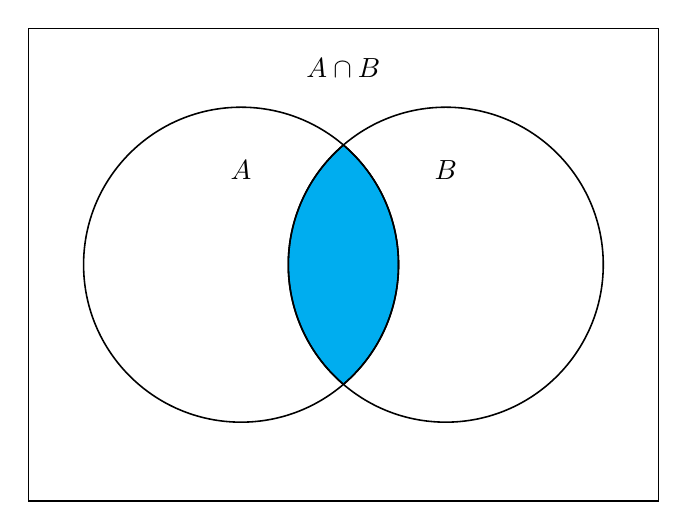
\begin{tikzpicture}[line width=0.2mm]
    % Coordinates for the centers of the circles.
    \coordinate (C1) at (-1.3, 0);
    \coordinate (C2) at ( 1.3, 0);

    % Coordinates for the labels.
    \coordinate (A) at (-1.3, 1.2);
    \coordinate (B) at ( 1.3, 1.2);
    \coordinate (I) at ( 0.0, 2.5);

    % Rectangle indicating the universe set.
    \draw (-4, -3) rectangle (4, 3);

    % Fill in the circle with cyan.
    \draw[fill=cyan] (0, -1.51987) arc(-49.46:49.46:2) arc(130.54:229.46:2);

    % Give outlines to the circles.
    \draw (C1) circle (2);
    \draw (C2) circle (2);

    % Labels.
    \node at (A) {$A$};
    \node at (B) {$B$};
    \node at (I) {$A\cap{B}$};
\end{tikzpicture}
            \caption{Venn Diagram for Intersection}
            \label{fig:Intersection_of_Two_Sets}
        \end{figure}
        We can extend this further and define the intersection over any
        collection of sets.
        \begin{ltheorem}{Existence of the Intersection of Sets}
                        {thm:Existence_of_Arbitrary_Intersetions}
            If $\mathcal{O}$ is a set, then there exists a set \gls{intersectO}
            such that for all $x$ it is true that $x\in\bigcap\mathcal{O}$ if
            and only if $x\in\bigcup\mathcal{O}$ and for all
            $\mathcal{U}\in\mathcal{O}$ it is true that $x\in\mathcal{U}$.
        \end{ltheorem}
        \begin{proof}
            For by Thm.~\ref{thm:Existence_of_Unions} there is a set
            $\bigcup\mathcal{O}$ such that for all $x$ it is true that
            $x\in\bigcup\mathcal{O}$ if and only if there exists a
            $\mathcal{U}\in\mathcal{O}$ such that $x\in\mathcal{U}$. Let
            $P$ be the proposition \textit{True if for all}
            $\mathcal{U}\in\mathcal{O}$ \textit{it is true that}
            $x\in\mathcal{U}$, \textit{false otherwise}. Then by the
            axiom schema of specification
            (Ax.~\ref{ax:Axiom_Schema_of_Specification}), there exists the set:
            \begin{equation}
                \bigcap\mathcal{O}
                =\Big\{\,x\in\bigcup\mathcal{O}
                    \;|\;P(x)\,\Big\}
            \end{equation}
            But then $x\in\bigcap\mathcal{O}$ if and only if
            $x\in\bigcup\mathcal{O}$ and $P(x)$ is true. That is,
            $x\in\bigcap\mathcal{O}$ if and only if $x\in\bigcup\mathcal{O}$
            and for all $\mathcal{U}\in\mathcal{O}$ it is true that
            $x\in\mathcal{U}$.
        \end{proof}
        It is common to consider some \textit{universal} set, of which all
        other sets of current consideration are drawn from. Using this the
        definition of arbitrary intersection is defined as the subset of
        this universal set such that every element of this subset is
        contained in every element of the arbitrary collection. One may then
        ask what would happen if the collection is empty. Using this
        definition the intersection would be the entire universal set
        in a vacuous sense. That is, there would be no $x$ in the universe
        that fails the definition of the intersection over an empty
        collection, and thus the intersection is everything. Letting $X$
        denote our universe, we obtain:
        \begin{equation}
            \emptyset=\bigcup_{\mathcal{U}\in\emptyset}\mathcal{U}
                \subseteq\bigcap_{\mathcal{U}\in\emptyset}\mathcal{U}
            =X
        \end{equation}
        It seems like unions should always be bigger. Indeed, for any
        non-empty collection, the intersection over the collection is a
        subset of the union over the collection. Because of this we do
        not adopt this definition of the intersection over a collection,
        but rather require in our construction the use of the union over
        the collection, and then use the axiom schema of specification to
        pick the subset of all elements of the union that belong to every
        element of the collection. Thus:
        \begin{equation}
            \bigcap_{\mathcal{U}\in\emptyset}\mathcal{U}
            \subseteq\bigcup_{\mathcal{U}\in\emptyset}\mathcal{U}
            =\emptyset
        \end{equation}
        And from this we conclude the intersection is empty as well.
        \begin{fdefinition}{Intersection Over a Collection}
                           {Intersection_Over_a_Collection}
            The \gls{intersection over a set} $\mathcal{O}$
            of sets is the set \gls{intersectO} defined by:
            \begin{equation*}
                \bigcap_{\mathcal{U}\in\mathcal{O}}\mathcal{U}
                =\Big\{\,x\in\bigcup_{\mathcal{U}\in\mathcal{O}}\mathcal{U}
                    \;\Big|\;x\in\mathcal{U}\textrm{ for all }
                    \mathcal{U}\in\mathcal{O}\,\Big\}
            \end{equation*}
            That is:
            \begin{equation*}
                \forall_{\mathcal{O}}\forall_{x}\bigg(
                    \Big(x\in\bigcap_{\mathcal{U}\in\mathcal{O}}\mathcal{U}\Big)
                    \Longleftrightarrow\Big(
                        \big(
                            x\in\bigcup_{\mathcal{U}\in\mathcal{O}}\mathcal{U}
                        \big)
                        \land\big(
                            \forall_{\mathcal{U}\in\mathcal{O}}
                            (x\in\mathcal{U})
                        \big)
                    \Big)
                \bigg)
            \end{equation*}
        \end{fdefinition}
        We can extend our Venn diagram for larger collections as well
        (see Fig.~\ref{fig:Intersection_of_Three_Sets}).
        \begin{figure}[H]
            \centering
            \begin{tikzpicture}
    % Coordinates for the centers of the circles.
    \coordinate (C1) at (-1.3,  0.00);
    \coordinate (C2) at ( 1.3,  0.00);
    \coordinate (C3) at ( 0.0, -2.15);

    \coordinate (O)  at ( 0.0000, -0.7500);
    \coordinate (P1) at ( 0.6817, -0.2697);
    \coordinate (P2) at (-0.6817, -0.2697);
    \coordinate (P3) at ( 0.0000, -1.5198);

    % Coordinates for the labels.
    \coordinate (A) at (-1.3, 1.2);
    \coordinate (B) at ( 1.3, 1.2);
    \coordinate (C) at ( 0.0, -3.5);
    \coordinate (U) at ( 0.0, 2.5);

    % Rectangle indicating the universe set.
    \draw (-4, -4.5) rectangle (4, 3.3);

    % Fill in the intersection with cyan.
    \draw[fill=cyan, draw=none] (P1) arc(70.07:109.93:2)
                                     arc(187.8:229.50:2)
                                     arc(310.54:352.25:2);

    % Give outlines to the circles.
    \draw (C1) circle (2);
    \draw (C2) circle (2);
    \draw (C3) circle (2);

    % Labels.
    \node at (A) {$A$};
    \node at (B) {$B$};
    \node at (C) {$C$};
    \node at (U)
        {\Large{$\underset{\mathcal{U}\in\{A,B,C\}}{\bigcap}\mathcal{U}$}};
\end{tikzpicture}
            \caption{The Intersection of Three Sets}
            \label{fig:Intersection_of_Three_Sets}
        \end{figure}
        Much the way we've defined what it means for two sets to be disjoint, we
        can extend this to arbitrary collections. We'll say that a collections
        of sets is mutually disjoint if all distinct elements of the collection
        have empty intersection. That is, all distinct pairs are disjoint.
        \begin{fdefinition}{Mutually Disjoint Collection of Sets}
                           {Mutually_Disjoint_Collection_of_Sets}
            A mutually disjoint collection of sets is a set $\mathcal{O}$ such
            that for all $A,B\in\mathcal{O}$ such that $A\ne{B}$ it is true that
            $A\cap{B}=\emptyset$. That is, for all distinct elements
            $A,B\in\mathcal{O}$ it is true that $A$ and $B$ are
            \glslink{disjoint sets}{disjoint}.
            \index{Mutually Disjoint Collection}
        \end{fdefinition}
        The term pairwise disjoint\index{Pairwise Disjoint} is also frequently
        used in measure theory and probability. As such, one might guess that
        the notion has a fair amount of use in these subjects. Next on the list
        of axioms is that of \textit{regularity}.
        \begin{faxiom}{Axiom of Regularity}{Axiom_of_Regularity}
            If $A$ is a non-empty set, then there is an element $B\in{A}$
            such that $A\cap{B}=\emptyset$.\index{Axiom!of Regularity}
            \begin{equation*}
                \forall_{A}(\exists_{x\in{A}})\Rightarrow
                \exists_{y}:\Big((y\in{A})\land
                \big((y\cap{A})=\emptyset\big)\Big)
            \end{equation*}
        \end{faxiom}
        This axiom is often seen as unnecessary by many working mathematicians
        and indeed it's use seems to only lie in set theory and foundations.
        That is, unlike the axioms of choice and union which are widely
        applicable to analysis and topology, regularity seems to only be useful
        to set theorists. This is not entirely true if one really pays attention
        to the details. Often we are presented some object $X$, perhaps a
        topological space, or an algebraic structure like a group, and we need
        to extend this object to a larger collection. One concrete example comes
        from topology when we have a \textit{non-compact} space $(X,\tau)$ and
        we want to find a \textit{compact} space $(\tilde{X},\tilde{\tau})$ that
        contains our original space. In the construction we add a single point
        to $(X,\tau)$ called \textit{infinity}, and label it $\infty$. But what
        if the symbol $\infty$ already belongs to $X$? How do we find a new
        object that is guarenteed not to lie in $X$? The axiom of regularity
        allows us to show that $\{X\}$ does not lie in $X$, for any set $X$, and
        thus we can take this to be our new point. This, and many similar
        constructions, rely on the axiom of regularity to guarentee that our
        reasoning is not ultimately circular.
        \par\hfill\par
        Regardless of the axioms application, its existence is vital to support
        the claim that ZFC is a good system to base mathematics on. We will
        combine this with pairing to prove that for any set $A$ it is true that
        $A\notin{A}$. That is, Zermelo-Fraenkel set theory is free of Russell's
        paradox\index{Russell's Paradox}.
        \begin{theorem}
            \label{thm:Anti_Russells_Paradox}%
            If $A$ is a set, then $A\notin{A}$.
        \end{theorem}
        \begin{proof}
            For if $A$ is a set, then $\{A\}$ is a set
            (Thm.~\ref{thm:Existence_of_Set_Containing_Set}). But since
            $A\in\{A\}$, $\{A\}$ is a non-empty set
            (Def.~\ref{def:Non_Empty_Set}). Thus by the axiom of regularity
            (Ax.~\ref{ax:Axiom_of_Regularity}) there is a set $B\in\{A\}$ such
            that $B\cap\{A\}=\emptyset$. But $B\in\{A\}$ if and only if
            $B=A$, and therefore $A\cap\{A\}=\emptyset$. Thus, by the axiom of
            the empty set (Ax.~\ref{ax:Axiom_of_the_Empty_Set}), for all $x$ it
            is true that $x\notin{A}\cap\{A\}$ and therefore
            $A\notin{A}\cap\{A\}$. But $A\in\{A\}$ and therefore
            $A\notin{A}$ (Thm.~\ref{thm:Lemma_for_Anti_Russells_Paradox}).
        \end{proof}
        \begin{theorem}
            \label{thm:Containment_NEqual_Underlying_Set}%
            If $A$ and $B$ are sets and if $A\in{B}$, then $A\ne{B}$.
        \end{theorem}
        \begin{proof}
            For $A\notin{A}$ (Thm.~\ref{thm:Anti_Russells_Paradox}) and
            $A\in{B}$ and therefore it is not true that for all $x$, $x\in{A}$
            if and only if $x\in{B}$. Therefore, by the Axiom of
            Extensionality (Ax.~\ref{ax:Axiom_of_Extensionality}), $A\ne{B}$.
        \end{proof}
        \begin{theorem}
            \label{thm:Cor_of_Containment_NEqual_Underlying_Set}%
            If $A$ is a set, then $A\ne\{A\}$.
        \end{theorem}
        \begin{proof}
            For if $A$ is a set, then $A\notin{A}$
            (Thm.~\ref{thm:Anti_Russells_Paradox}). But if $A$ is a set, then
            $\{A\}$ is a set (Thm.~\ref{thm:Existence_of_Set_Containing_Set}).
            But $A\in\{A\}$, and thus $A\ne\{A\}$
            (Thm.~\ref{thm:Containment_NEqual_Underlying_Set}).
        \end{proof}
        These quick theorems will eventually prove the well known result that
        $0\ne{1}$. It also shows us that there is no set of all
        sets\index{Set!of All Sets}.
    \subsection{The Axiom of the Power Set}
        Continuing in our goal of constructing order, we move on to the
        Cartesian product\index{Cartesian Product} of two sets $A$ and $B$. This
        is the collection of all ordered pairs $(a,b)$ such that $a\in{A}$ and
        $b\in{B}$. To prove such a set exists requires the
        \textit{axiom of the power set}.
        \begin{faxiom}{Axiom of the Power Set}{Axiom_of_the_Power_Set}
            If $A$ is a set, then there exists a set $\mathscr{P}$ such that
            for all $x\subseteq{A}$ it is true that $x\in\mathscr{P}$.
            \index{Axiom!of the Power Set}
            \begin{equation*}
                \forall_{A}\exists_{\mathscr{P}}:
                \forall_{x}\Big((x\subseteq{X})\Rightarrow(x\in\mathscr{P})\Big)
            \end{equation*}
        \end{faxiom}
        Again, much like the axiom of union and the axiom of pairing, this
        set may be bigger than we would like. We wish to find a set, called
        the \textit{power set}, that contains all of the subsets of a given
        set $A$ and nothing else. Combining the axiom of the power set
        with the axiom schema of specification gives us such existence.
        \begin{ltheorem}{Existence of the Power Set}
                        {Existence_of_the_Power_Set}
            If $A$ is a set, then there exists a set \gls{powersetsymb}
            such that for all $x$ it is true that $x\in\mathcal{P}(A)$ if and
            only if $x\subseteq{A}$.\index{Set!Power Set}
        \end{ltheorem}
        \begin{proof}
            For by the axiom of the power set
            (Ax.~\ref{ax:Axiom_of_the_Power_Set}) there is a set $\mathscr{P}$
            such that for all $x\subseteq{A}$ it is true that $x\in\mathscr{P}$.
            Let $P$ be the proposition \textit{true if} $x\subseteq{A}$,
            \textit{false otherwise}. By the axiom schema of specification
            (Ax.~\ref{ax:Axiom_Schema_of_Specification}), there is a set
            $\mathcal{P}(A)$ such that:
            \begin{equation}
                \mathcal{P}(A)=\{\,x\in\mathscr{P}(A)\;|\;P(x)\,\}
            \end{equation}
            But if $P(x)$ is true, then $x$ is a subset of $A$, and therefore
            $x\in\mathscr{P}(A)$. Thus $x\in\mathcal{P}(A)$ if and only if
            $x\subseteq{A}$.
        \end{proof}
        With this we now define the \textit{power set} of a given set.
        \newpage
        \begin{fdefinition}{Power Set}{Power_Set}
            The \gls{power set} of a \gls{set} $A$ is the set $\mathcal{P}(A)$
            defined by:\index{Power Set}\index{Set!Power Set}
            \begin{equation*}
                \mathcal{P}(A)=\{\,x\;|\;x\subseteq{X}\,\}
            \end{equation*}
            That is, the set of all subsets of $X$.
            \begin{equation*}
                \forall_{A}\forall_{B}\Big(B\in\mathcal{P}(A)\Longleftrightarrow
                    B\subseteq{A}\Big)
            \end{equation*}
        \end{fdefinition}
        Again, there is some abuse of our set-builder notation, but
        Thm.~\ref{thm:Existence_of_the_Power_Set} justifies such a definition.
        The power set of a set is a crucial construction for when one discusses
        the \textit{cardinality} of sets, denoted $\textrm{Card}(A)$. This
        describes the \textit{size} of a set in a very precise manner. A theorem
        that will eventually be proved known as
        \textit{Cantor's Theorem}\index{Theorem!Cantor's Power Set Theorem}
        shows that the power set of a set is always strictly \textit{larger}
        than the original set. That is:
        \begin{equation}
            \textrm{Card}(A)<\textrm{Card}\big(\mathcal{P}(A)\big)
        \end{equation}
        This will be made precise soon enough. The axiom of the power set allows
        us to build \textit{larger} sets from a given set. This creates a
        paradoxical heirarchy of infinities. Starting with the \textit{smallest}
        infinity, the natural numbers $\mathbb{N}$, we can create a
        significantly larger set by considering $\mathcal{P}(\mathbb{N})$. We
        can continue and consider $\mathcal{P}(\mathcal{P}(\mathbb{N}))$, and
        there's no reason to stop there. At each step we create a new, massively
        larger set. This is both unintuitive and paradoxical and as such some
        may choose to reject it. This axiom is vital in the discussion of
        topology and measure theory, and so we choose to accept it as true.
        \begin{example}
            If $A=\{1,2\}$, then the power set is:
            \begin{equation}
                \mathcal{P}(A)=\big\{\,\emptyset,\,\{1\},\,\{2\},\,
                    \{1,2\}\,\big\}
            \end{equation}
            We must consider the empty set since $\emptyset\subseteq{A}$.
            Now suppose $A=\{1,2,3\}$:
            \begin{equation}
                \powset(A)=\big\{\,\emptyset,\,\{1\},\,\{2\},\,\{3\},\,
                    \{1,2\},\,\{1,3\},\,\{2,3\},\,\{1,2,3\}\,\big\}
            \end{equation}
            We see that a set with 2 elements has a power set with 4 elements
            and a set with 3 elements has a power set with 8. This pattern
            continues for finite sets and if $A$ has $n$ elements, then
            $\mathcal{P}(A)$ has $2^{n}$ elements.
        \end{example}
        \begin{example}
            Suppose we have two variables $a,b$ and the set $A=\{a,b\}$. We can
            compute the power set of $A$ as follows:
            \begin{equation}
                \powset{A}=\big\{\,\emptyset,\,\{a\},\,\{b\},\,A\,\big\}
            \end{equation}
            much like the previous example, we see that the power set of a set
            with 2 elements has $2^{2}=4$ elements.
        \end{example}
        \begin{example}
            Let $A=\{a_{1},\dots,a_{n}\}$, where all of the elements $a_{k}$ are
            distinct. To count the total number of subsets we first note that
            there is one set that contains zero elements, the empty set. Next,
            there are $n$ subsets that contain one element, these are the sets
            $\{a_{k}\}$. There are $n(n-1)/2$ sets that contain two elements,
            $\{a_{i},a_{j}\}$, such that $i\ne{j}$. Continuing, we see that
            there are $\binom{n}{k}$ subsets that contain $k$ elements, where
            $\binom{n}{k}$ is the \textit{binomial coefficient}%
            \index{Binomial Coefficient}. This is defined in terms of the
            factorial function:
            \begin{subequations}
                \begin{align}
                    \binom{n}{k}
                    &=\frac{n!}{k!(n-k)!}\\
                    &=\frac{n\cdot(n-1)\cdots{2}\cdot{1}}
                        {k\cdot(k-1)\cdots{2}\cdot{1}\cdot(n-k)
                        \cdot(n-k-1)\cdots{2}\cdot{1}}\\
                    &=\frac{n\cdot(n-1)\cdots\cdot(n-k+1)}
                        {k\cdot(k-1)\cdots{2}\cdot{1}}
                \end{align}
            \end{subequations}
            To avoid undefined ratios, we define $0!=1$. Note then that
            $\binom{n}{n}=1$. This says that the number of ways to choose $n$
            element subsets from $A$ is 1. This makes sense since the only $n$
            element subset of $A$ is the entirety of $A$! To compute the size of
            $\mathcal{P}(A)$ it now suffices to sum over all of these binomial
            coefficients. Such a task can be achieved by invoking the
            \textit{binomial theorem}\index{Theorem!Binomial Theorem}. Given
            a positive integer $n$ and two real numbers $x$ and $y$, the
            binomial theorem states that:
            \begin{subequations}
                \begin{align}
                    (x+y)^{n}
                    &=\sum_{k=0}^{n}\binom{n}{k}x^{n-k}y^{k}\\
                    &=\binom{n}{0}x^{n}+\binom{n}{1}x^{n-1}y+\cdots+
                        \binom{n}{n-1}xy^{n-1}+\binom{n}{n}y^{n}
                \end{align}
            \end{subequations}
            Here, the notation $\Sigma$ is simply shorthand for denoting a long
            sum. For example:
            \par
            \begin{subequations}
                \begin{minipage}[b]{0.49\textwidth}
                    \centering
                    \begin{equation}
                        \sum_{n=1}^{3}n=1+2+3=6
                    \end{equation}
                \end{minipage}
                \hfill
                \begin{minipage}[b]{0.49\textwidth}
                    \centering
                    \begin{equation}
                        \sum_{n=1}^{3}n^{2}=1+2^{2}+3^{2}=14
                    \end{equation}
                \end{minipage}
            \end{subequations}
            \par\vspace{2.5ex}
            Setting $x=y=1$, we obtain:
            \begin{equation}
                2^{n}=\sum_{k=0}^{n}\binom{n}{k}
            \end{equation}
            and this is precisely the number of elements of $\mathcal{P}(A)$.
        \end{example}
        \begin{example}
            When we consider the case of an \textit{infinite} set $A$ we have
            that $\mathcal{P}(A)$ is a strictly larger set and this creates a
            paradoxical heirarchy of infinities. The smallest heirarchy is
            that of the \textit{countable} infinite sets, like $\mathbb{N}$.
            Everything larger is called \textit{uncountable}. It will be
            shown that the following is true:
            \begin{equation}
                \Card\big(\mathcal{P}(\mathbb{N})\big)=
                \Card(\mathbb{R})
            \end{equation}
            where again $\mathbb{N}$ denotes the non-negative integers and
            $\mathbb{R}$ denotes the set of all \textit{real} numbers. We
            can loosely show this by using the binary representation of real
            numbers. A real number may be thought of as an infinite decimal.
            For example, $\pi=3.1415926\dots$ and $1=1.000\dots$ We can
            also represent real numbers as a sequence of zeroes and ones and
            this is the \textit{binary} representation. For
            $A\subseteq\mathbb{N}$ and let $r_{A}=0.n_{1}n_{2}\hdots$ where:
            \begin{equation}
                n_{i}=
                \begin{cases}
                    0,&i\notin{A}\\
                    1,&i\in{A}
                \end{cases}
            \end{equation}
            Thus for each $A\in\mathcal{P}(\mathbb{N})$ there is a real
            number $r_{A}$ such that $0\leq{r}_{A}\leq{1}$ that is
            associated with it, and moreover to every real number between
            zero and one there is a subset of $\mathbb{N}$ associated with
            it. The tricky numbers to see are zero and one, but note that
            $r_{\emptyset}$ is associated to 0 and $r_{\mathbb{N}}$ gets
            paired with 1. To show that $\mathbb{R}$ and
            $\mathcal{P}(\mathbb{N})$ are the same size requires us to
            refine this association so that every element of
            $\mathcal{P}(\mathbb{N})$ uniquely corresponds to an element of
            $\mathbb{R}$, and vice-versa.
        \end{example}
    \subsection{Cartesian Products and Functions}
        Previously we've introduced ordered pairs and the notion of the power
        set. We can use both of these concepts to define and prove the existence
        of \textit{Cartesian products}. Intuitively we want to define
        $A\times{B}$ to be the set of all ordered pairs $(a,b)$ where $a\in{A}$
        and $b\in{B}$:
        \begin{equation}
            A\times{B}=\big\{\,(a,\,b)\;|\;a\in{A}\textrm{ and }b\in{B}\,\big\}
        \end{equation}
        But recalling Def.~\ref{def:Ordered_Pairs}, ordered pairs are sets
        of the form $\{\{a\},\{a,b\}\}$. Thus elements of $A\times{B}$ are
        contained in the power set of the power set of $A\cup{B}$:
        \begin{equation}
            A\times{B}\subseteq\mathcal{P}\big(\mathcal{P}(A\cup{B})\big)
        \end{equation}
        We can combine the axiom of the power set with the axiom schema of
        specification to obtain the existence of the Cartesian product of
        two sets.\index{Axiom!of the Power Set}
        \index{Axiom!Schema of Specification}
        \begin{theorem}
            \label{thm:Ordered_Pair_Subset_of_Power_Set}%
            If $A$ and $B$ are sets, if $a\in{A}$ and $b\in{B}$, then
            $(a,b)\subseteq\mathcal{P}(A\cup{B})$.
        \end{theorem}
        \begin{proof}
            For if $a\in{A}$ and $b\in{B}$, then
            $(a,b)=\{\,\{\,a\,\},\,\{\,a,\,b\,\}\,\}$
            (Def.~\ref{def:Ordered_Pairs}). But if $a\in{A}$, then $a\in{A}$
            or $a\in{B}$, and thus $a\in{A}\cup{B}$
            (Def.~\ref{def:Union_of_Two_Sets}). But then
            $\{\,a\,\}\subseteq{A}\cup{B}$ (Def.~\ref{def:Subsets}). But if
            $b\in{B}$, then $b\in{A}$ or $b\in{B}$, and thus $b\in{A}\cup{B}$
            (Def.~\ref{def:Union_of_Two_Sets}). But then
            $\{\,a,\,b\,\}\subseteq{A}\cup{B}$ (Def.~\ref{def:Subsets}).
            But then $\{\,a\,\}\subseteq{A}\cup{B}$ and
            $\{\,a,\,b\,\}\subseteq{A}\cup{B}$, and thus
            $(a,b)\subseteq\mathcal{P}(A\cup{B})$ (Def.~\ref{def:Power_Set}).
        \end{proof}
        \begin{ltheorem}{Existence of the Cartesian Product}
                        {Existence_of_the_Cartesian_Product}
            If $A$ and $B$ are sets, then there exists a set $A\times{B}$
            such that, for all $z$, $z\in{A}\times{B}$ if and only if there
            is an $a\in{A}$ and $b\in{B}$ such that $z=(a,b)$.
            \index{Cartesian Product}
        \end{ltheorem}
        \begin{proof}
            For if $A$ and $B$ are sets, then $A\cup{B}$ is a set
            (Thm.~\ref{thm:Union_of_Two_Sets_Exists}). But if $A\cup{B}$ is a
            set, then $\mathcal{P}(A\cup{B})$ is a set
            (Thm.~\ref{thm:Existence_of_the_Power_Set}), where $\mathcal{P}(X)$
            denotes the power set of $X$. But if $\mathcal{P}(A\cup{B})$ is a
            set, then $\mathcal{P}(\mathcal{P}(A\cup{B}))$ is a set
            (Thm.~\ref{thm:Existence_of_the_Power_Set}). But then
            $z\in\mathcal{P}(\mathcal{P}(A\cup{B}))$ if and only if
            $z\subseteq\mathcal{P}(A\cup{B})$ (Def.~\ref{def:Power_Set}).
            But if $a\in{A}$ and $b\in{B}$, then
            $(a,b)\subseteq\mathcal{P}(A\cup{B})$
            (Thm.~\ref{thm:Ordered_Pair_Subset_of_Power_Set}), and therefore
            $(a,b)\in\mathcal{P}(\mathcal{P}(A\cup{B}))$. Let $P$ be the
            proposition \textit{True if there exists} $a\in{A}$ \textit{and}
            $b\in{B}$ \textit{such that} $z=(a,b)$, \textit{false otherwise}.
            Then by the axiom schema of specification
            (Ax.~\ref{ax:Axiom_Schema_of_Specification}), there exists a
            set $A\times{B}$ such that:
            \begin{equation}
                A\times{B}=
                \{\,z\in\mathcal{P}\big(\mathcal{P}(A\cup{B})\big)\;|\;
                    P(z)\,\}
            \end{equation}
            But it was proved that $P(z)$ implies that
            $z\in\mathcal{P}(\mathcal{P}(A\cup{B}))$. Thus $z\in{A}\times{B}$
            if and only if there exists $a\in{A}$ and $b\in{B}$
            such that $z=(a,b)$.
        \end{proof}
        \begin{fdefinition}{Cartesian Product of Two Sets}
                           {Cartesian_Product_of_Two_Sets}
            The \gls{Cartesian product} of two \glspl{set} $A$ and $B$ is the
            set:\index{Cartesian Product}
            \begin{equation*}
                A\times{B}
                =\{\,(a,\,b)\;|\;a\in{A}\textrm{ and }b\in{B}\,\}
            \end{equation*}
            Formally:
            \begin{equation*}
                \forall_{A}\forall_{B}\forall_{z}\Big(
                    (z\in{A}\times{B})\Longleftrightarrow
                    \big(\exists_{x\in{A}}\land\exists_{y\in{B}}:z=(x,y)\big)
                \Big)
            \end{equation*}
        \end{fdefinition}
        Note that since, in general, $(a,b)\ne(b,a)$, it is generally true that
        $A\times{B}\ne{B}\times{A}$. Indeed, equality occurs if and only if
        $A=B$ (or if either set is empty).
        \begin{fexample}{Basic Cartesian Products}{Basic_Cartesian_Products}
            Let $A$ and $B$ be sets defined as follows:
            \par
            \begin{subequations}
                \begin{minipage}[b]{0.49\textwidth}
                    \centering
                    \begin{equation}
                        A=\{\,1,\,2,\,3\,\}
                    \end{equation}
                \end{minipage}
                \hfill
                \begin{minipage}[b]{0.49\textwidth}
                    \centering
                    \begin{equation}
                        B=\{\,a,\,b\,\}
                    \end{equation}
                \end{minipage}
            \end{subequations}
            \par\vspace{2.5ex}
            Let's compute $A\times{B}$ and $B\times{A}$. From the definition
            (Def.~\ref{def:Cartesian_Product_of_Two_Sets}) we have:
            \begin{equation}
                A\times{B}=\{\,(a,b)\;|\;a\in{A}\textrm{ and }b\in{B}\,\}
            \end{equation}
            Using this, we can compute:
            \begin{equation}
                A\times{B}=\big\{\,(1,a),\,(2,a),\,(3,a),\,
                                   (1,b),\,(2,b),\,(3,b)\,\big\}
            \end{equation}
            Computing $B\times{A}$, we have:
            \begin{equation}
                B\times{A}=\big\{\,(a,\,1),\,(a,\,2),\,(a,\,3),\,
                                   (b,\,1),\,(b,\,2),\,(b,\,3)\,\big\}
            \end{equation}
            Now if we suppose that $a$ is not equal to 1, then we see that
            $(a,1)$ is a different element than $(1,a)$, and thus $A\times{B}$
            is not equal to $B\times{A}$. Next, compute $A\times{A}$:
            \begin{equation}
                \begin{split}
                    A\times{A}=\Big\{\,(1,1),\,(1,2),\,&(1,3),
                                       (2,1),\,(2,2),\,\\&(2,3),
                                       (3,1),\,(3,2),\,(3,3)\,\Big\}
                \end{split}
            \end{equation}
            And finally $B\times{B}$:
            \begin{equation}
                B\times{B}=\big\{\,(a,\,a),\,(a,\,b),
                                 \,(b,\,a),\,(b,\,b)\,\big\}
            \end{equation}
            Equality of $A\times{B}$ and $B\times{A}$ is achieved if and only
            if $A=B$, or if either set is the empty set.
        \end{fexample}
        Note that in Ex.~\ref{ex:Basic_Cartesian_Products}, the \textit{size}
        of the Cartesian product of two sets was simply the product of the
        number of elements of the constituent sets. That is, we see that $A$
        has three elements and $B$ has two elements, but also that
        $A\times{B}$ has six elements. Moreover, $A\times{A}$ has nine
        elements and $B\times{B}$ has four. This pattern holds for the
        Cartesian products of any two \textit{finite} sets.
        \index{Set!Finite}
        \par\hfill\par
        It is common to consider the Cartesian product of a set with itself.
        That is, given a set $A$, we are often interested in $A\times{A}$. We
        denote this by writing $A^{2}$. One such example is when we consider
        the set of real numbers $\mathbb{R}$. The Cartesian product
        $\mathbb{R}^{2}$ is called the \textit{Euclidean Plane}, or the
        \textit{Cartesian Plane}\index{Euclidean Plane}\index{Cartesian Plane},
        after Euclid of Alexandria\index{Euclid of Alexandria} and Ren\'{e}
        Descartes\index{Descartes, Ren\'{e}}. This is because $\mathbb{R}^{2}$
        is used to model both planar geometry and analytical geometry, of which
        Euclid and Descartes were pioneers of, respectively. The term Cartesian
        products is in honor of Ren\'{e} Descartes, as well. Let $\mathbb{R}$
        denote the set of real numbers, and let $A=\mathbb{R}$ and
        $B=\mathbb{R}$. Then we have:
        \begin{equation}
            A\times{B}=\mathbb{R}\times\mathbb{R}\equiv\mathbb{R}^{2}
        \end{equation}
        Where the symbol \gls{equiv} means that $\mathbb{R}^{2}$ is defined by
        this expression. Using the definition of Cartesian products
        (Def.~\ref{def:Cartesian_Product_of_Two_Sets}), we obtain:
        \begin{equation}
            \mathbb{R}^{2}=\{\;(x,y)\,:\,x\in\mathbb{R}
                               \textrm{ and }y\in\mathbb{R}\;\}
        \end{equation}
        That is, $\mathbb{R}^{2}$ is the set of all ordered pairs of real
        numbers. The first term is called the $x$ coordinate, and similarly the
        second term is called the $y$ coordinate. We envision this as a
        \textit{plane} of points, each one corresponding to an ordered pair
        $(x,y)$. This is depicted in Fig.~\ref{fig:Cartesian_Plane}.
        \begin{figure}[H]
            \centering
            %--------------------------------Dependencies----------------------------------%
%   tikz                                                                       %
%       arrows.meta                                                            %
%-------------------------------Main Document----------------------------------%
\begin{tikzpicture}[%
    >=Latex,
    line width=0.2mm,
    line cap=round,
    font=\Large
]
    % Coordinates for the points.
    \coordinate (x) at (2.2, 0.0);
    \coordinate (y) at (0.0, 2.9);
    \coordinate (z) at (2.2, 2.9);

    % Draw a grid.
    \draw[style=help lines] (-0.3, -0.3) grid (7.9, 7.9);

    % Axes.
    \begin{scope}[thick]
        \draw[->] (-0.3, 0) to (8.4, 0) node [above] {$\mathbb{R}$};
        \draw[->] (0, -0.3) to (0, 8.4) node [right] {$\mathbb{R}$};
    \end{scope}

    % Draw dashed lines to the point.
    \begin{scope}[densely dashed]
        \draw (x) to (z);
        \draw (y) to (z);
    \end{scope}

    % Draw dots marking the various points.
    \draw[fill=black] (x) circle (0.6mm);
    \draw[fill=black] (y) circle (0.6mm);
    \draw[fill=black] (z) circle (0.6mm);

    % Label the points x, y, and the dot (x,y) in the plane.
    \node at (x) [below=0.1]     {$x$};
    \node at (y) [left=0.1]      {$y$};
    \node at (z) [above right]   {$(x,\,y)$};
\end{tikzpicture}
            \caption{The Cartesian Plane $\mathbb{R}^{2}$}
            \label{fig:Cartesian_Plane}
        \end{figure}
        Consider further the set $\mathbb{N}^{2}$. That is, letting
        $\mathbb{N}$ denote the set of natural numbers
        (Eqn.~\ref{eqn:Natural_Numbers_Ellipses}), letting $A=\mathbb{N}$ and
        $B=\mathbb{N}$ we have:\index{Integer Lattice}
        \begin{equation}
            A\times{B}=\mathbb{N}\times\mathbb{N}\equiv\mathbb{N}^{2}
        \end{equation}
        Again using the definition of Cartesian products
        (Def.~\ref{def:Cartesian_Product_of_Two_Sets}), we have:
        \begin{equation}
            \mathbb{N}^{2}=
            \{\,(n,\,m)\;|\;n\in\mathbb{N}\textrm{ and }m\in\mathbb{N}\,\}
        \end{equation}
        We can visualize this as a subset of $\mathbb{R}^{2}$ by drawing a
        lattice of points in the Cartesian plane
        (Fig.~\ref{fig:Lattice_Cart_Prod_of_N_with_N}).
        \begin{figure}[H]
            \centering
            %--------------------------------Dependencies----------------------------------%
%   tikz                                                                       %
%       arrows.meta                                                            %
%-------------------------------Main Document----------------------------------%
\begin{tikzpicture}[%
    >=Latex,
    line width=0.2mm,
    line cap=round
]

    % Axes.
    \begin{scope}[thick, font=\Large]
        \draw[->] (0, 0) to (8.4, 0) node [above] {$\mathbb{N}$};
        \draw[->] (0, 0) to (0, 8.4) node [right] {$\mathbb{N}$};
    \end{scope}

    \foreach\x in{1, 2, 3, 4, 5, 6, 7, 8}{
        \foreach\y in{1, 2, 3, 4, 5, 6, 7, 8}{
            \draw[fill=black] (\x, \y) circle (0.2mm);
        }
        \draw (\x, -0.1) to (\x, 0.1) node [below=1ex] {$\x$};
        \draw (-0.1, \x) to (0.1, \x) node [left=1ex]  {$\x$};
    }
\end{tikzpicture}
            \caption{The Lattice $\mathbb{N}^{2}$}
            \label{fig:Lattice_Cart_Prod_of_N_with_N}
        \end{figure}
        This can then be consider a subset of the Euclidean plane
        $\mathbb{R}^{2}$. That is, at every ordered pair of integers $(m,n)$,
        we place a point in the Euclidean plane whose $x$ coordinate is $m$ and
        whose $y$ coordinate is $n$. We can also be more abstract and general in
        our examples. Consider the following sets:
        \par
        \begin{subequations}
            \begin{minipage}[b]{0.49\textwidth}
                \centering
                \begin{equation}
                    A=\{\,\textrm{Point, Line 1, Line 2}\,\}
                \end{equation}
            \end{minipage}
            \hfill
            \begin{minipage}[b]{0.49\textwidth}
                \centering
                \begin{equation}
                    B=\{\,\textrm{Point, Line}\,\}
                \end{equation}
            \end{minipage}
        \end{subequations}
        \par\vspace{2.5ex}
        We can visually represent the Cartesian product $A\times{B}$ by
        drawing $A$ in green and $B$ in red, as shown in
        Fig.~\ref{fig:Cartesian_Product_Example}. The Cartesian Product
        $A\times{B}$ is the set formed by connecting all of the points
        from $A$ and $B$ in the plane. This is shown in blue.
        \begin{figure}[H]
            \centering
            %--------------------------------Dependencies----------------------------------%
%   tikz                                                                       %
%       arrows.meta                                                            %
%-------------------------------Main Document----------------------------------%
\begin{tikzpicture}[%
    >=Latex,
    line width=0.2mm,
    line cap=round
]

    % Draw green to indicate the set A.
    \begin{scope}[green]

        % Draw some points.
        \draw[fill=green] (1, 0) circle (0.3mm);
        \draw[fill=green] (2, 0) circle (0.3mm);
        \draw[fill=green] (5, 0) circle (0.3mm);
        \draw[fill=green] (6, 0) circle (0.3mm);
        \draw[fill=green] (7, 0) circle (0.3mm);

        % Draw lines.
        \draw (2, 0) to (5, 0);
        \draw (6, 0) to (7, 0);
    \end{scope}

    % Draw red to denote the set B.
    \begin{scope}[red]

        % Draw in some points.
        \draw[fill=red] (0, 1) circle (0.3mm);
        \draw[fill=red] (0, 2) circle (0.3mm);
        \draw[fill=red] (0, 5) circle (0.3mm);

        % Draw a line.
        \draw (0, 2) to (0, 5);
    \end{scope}

    % Use blue to mark AxB (Cartesian product).
    \begin{scope}[blue]

        % Fill in points.
        \draw[fill=blue] (1, 1) circle (0.3mm);
        \draw[fill=blue] (1, 2) circle (0.3mm);
        \draw[fill=blue] (1, 5) circle (0.3mm);
        \draw[fill=blue] (2, 1) circle (0.3mm);
        \draw[fill=blue] (5, 1) circle (0.3mm);
        \draw[fill=blue] (6, 1) circle (0.3mm);
        \draw[fill=blue] (7, 1) circle (0.3mm);
        \draw[fill=blue] (2, 2) circle (0.3mm);
        \draw[fill=blue] (2, 5) circle (0.3mm);
        \draw[fill=blue] (5, 2) circle (0.3mm);
        \draw[fill=blue] (5, 5) circle (0.3mm);
        \draw[fill=blue] (6, 2) circle (0.3mm);
        \draw[fill=blue] (7, 2) circle (0.3mm);
        \draw[fill=blue] (6, 5) circle (0.3mm);
        \draw[fill=blue] (7, 5) circle (0.3mm);

        % Draw lines.
        \draw (1, 2) to (1, 5);
        \draw (2, 1) to (5, 1);
        \draw (6, 1) to (7, 1);

        % Fill in rectangles.
        \draw[fill=blue, opacity=0.4] (2, 2) to (5, 2) to (5, 5)
                                             to (2, 5) to cycle;
        \draw[fill=blue, opacity=0.4] (6, 2) to (7, 2) to (7, 5)
                                             to (6, 5) to cycle;
        \draw (2, 2) to (5, 2) to (5, 5) to (2, 5) to cycle;
        \draw (6, 2) to (7, 2) to (7, 5) to (6, 5) to cycle;
    \end{scope}
\end{tikzpicture}
            \caption[Cartesian Product of Two Sets]
                {The Cartesian Product of Two Sets. $A$ is
                 in \textcolor{green}{Green},
                 $B$ is in \textcolor{red}{red}, and
                 $A\times{B}$ is in \textcolor{blue}{blue}.}
            \label{fig:Cartesian_Product_Example}
        \end{figure}
        Cartesian products are not \textit{associative}%
        \index{Binary Operation!Associative}. That is, given three sets $A$,
        $B$, and $C$, there is no clear way to take the Cartesian
        product\index{Cartesian Product} of these since:
        \begin{equation}
            A\times(B\times{C})\ne(A\times{B})\times{C}
        \end{equation}
        To see this, note that the elements of $A\times(B\times{C})$ are
        ordered pairs of the form $\big(a,\,(b,\,c)\big)$, whereas elements of
        $(A\times{B})\times{C}$ are of the form $\big((a,\,b),\,c\big)$. When
        we write $A\times{B}\times{C}$ we really want ordered \textit{triples}
        of the form $(a,\,b,\,c)$.
        Much the way ordered pairs have been defined, we can modify Kuratowski's
        approach and define ordered triples\index{Ordered Triple} and ordered
        $n$ tuples\index{Ordered $n$ Tuple}. Rather than doing this we will use
        the language of functions to define higher order Cartesian products.
        \begin{fdefinition}{Functions}{Function}
            A \gls{function} from a \gls{set} $A$ to a set $B$ is a \gls{subset}
            $f\subseteq{A}\times{B}$, denoted $f:A\rightarrow{B}$, such that
            for all $x\in{A}$ there is a unique $y\in{B}$ such that
            $(x,y)\in{f}$. $A$ is called the domain of $f$
            and $B$ is called the codomain.\index{Function}
        \end{fdefinition}
        We're used to hearing that a function is a rule that assigns to an
        input value $x$ some output value $f(x)$. It may seem hard to justify,
        then, why we've defined a function as a subset of the Cartesian
        product. But note the requirement that for each $x\in{A}$ there is a
        \textit{unique} $y\in{B}$ such that $(x,y)\in{f}$. We call this unique
        element the \textit{image} of $x$ under the function $f$ and write
        $y=f(x)$. The condition that there is a unique such value $y$ to each
        $x$ is called the \textit{vertical line test}\index{Vertical Line Test}
        when graphing functions of the form $f:\mathbb{R}\rightarrow\mathbb{R}$
        (Fig.~\ref{fig:Function_R_to_R_Subset_Cart_Prod}). Simply, given such
        a function, if one draws a vertical line in the plane, then it must
        intersect the graph of $f$ once and only once. This provides a
        quick means of discerning functions from non-functions.
        \begin{lexample}{The Square Function}{Square_Function}
            If we can come up with some rule that assigns to every element
            $a\in{A}$ a unique element of $B$, then we can use this rule to
            define a function $f:A\rightarrow{B}$. Such a rule often comes
            in the form of a \textit{formula}\index{Formula}. We write the
            unique element that $a$ corresponds to as $f(b)$. For example, let
            $A=\mathbb{R}$ and let $B=\mathbb{R}$. We can define a function by
            the squaring formula:
            \begin{equation}
                f(x)=x\cdot{x}=x^{2}
            \end{equation}
            Once we know that $x^{2}$ gives a unique number
            (which will require some notion of arithmetic), we can define
            the function $f:\mathbb{R}\rightarrow\mathbb{R}$ by:
            \begin{equation}
                f=\{\,(x,\,x^{2})\in\mathbb{R}^{2}\;|\;x\in\mathbb{R}\,\}
            \end{equation}
            Usually we'll define functions by their formula's, rather than
            expressing them explicitly as subsets of the Cartesian product.
        \end{lexample}
        In the field of mathematical analysis we are often concerned with
        functions involving real numbers. For the sake of intuition, let
        us consider functions of the form $f:\mathbb{R}\rightarrow\mathbb{R}$.
        Any curve that we draw left-to-right, without picking up the pencil,
        will be a valid function.
        (See Fig.~\ref{fig:Function_R_to_R_Subset_Cart_Prod}).
        \begin{figure}[H]
            \centering
            %--------------------------------Dependencies----------------------------------%
%   xcolor                                                                     %
%   amssymb                                                                    %
%   tikz                                                                       %
%       arrows.meta                                                            %
%-------------------------------Main Document----------------------------------%
\begin{tikzpicture}[%
    >=Latex,
    line width=0.2mm,
    line cap=round,
    scale=1.2
]
    % Coorindates for the curve.
    \coordinate (P1) at (-4.00, -2.00);
    \coordinate (P2) at (-2.00, -3.00);
    \coordinate (P3) at ( 0.00,  0.00);
    \coordinate (P4) at ( 2.00,  3.00);
    \coordinate (P5) at ( 4.00,  3.90);

    % Draw a green mesh indicating the Cartesian plane.
    \foreach\x in {-40, -39, ..., 39}{
        \draw[draw=green, line width=0.1mm] (\x/10, -4) to (-4, \x/10);
        \draw[draw=green, line width=0.1mm] (4, \x/10)  to (\x/10, 4);
    }
    \draw[draw=green, line width=0.1mm] (4, 4)  to (4, 4);

    \begin{scope}[thick, font=\Large]
        \draw[<->] (-4.3,  0.0) to (4.3, 0.0) node [above] {$\mathbb{R}$};
        \draw[<->] ( 0.0, -4.3) to (0.0, 4.3) node [right] {$\mathbb{R}$};
    \end{scope}

    \draw[draw=blue] (P1) to [out=-30, in=150]  (P2)
                          to [out=-30, in=210]  (P3)
                          to [out=30,  in=180]  (P4)
                          to [out=0,   in=200]  (P5);
    \draw[fill=white, draw=white] 
        (1.3, 2.0) rectangle node {$\textcolor{blue}{f}$} (1.6, 1.4);
\end{tikzpicture}
            \caption[Example of a Function $f:\mathbb{R}\rightarrow\mathbb{R}$]
                    {Example of a function $f:\mathbb{R}\rightarrow\mathbb{R}$.
                     The Cartesian product $\mathbb{R}\times\mathbb{R}$ is
                     shown in \textcolor{green!80!black}{green}, and the
                     function $f\subseteq\mathbb{R}\times\mathbb{R}$ is shown
                     in \textcolor{blue}{blue}.}
            \label{fig:Function_R_to_R_Subset_Cart_Prod}
        \end{figure}
        Let $g\subseteq\mathbb{R}\times\mathbb{R}$ be defined as follows:
        \begin{equation}
            g=\big\{\,(x,\,y)\in\mathbb{R}^{2}\;|\;y^{2}=x\,\big\}
        \end{equation}
        It is tempting to label $g$ by writing $g(x)=\sqrt{x}$, but $g$ is
        not a function for it fails two of the requirements of a function.
        Firstly, for any $x>0$, there are two values $y_{1}$ and $y_{2}$
        whose square is equal to $x$. Indeed, if $y_{1}$ is one such value,
        then setting $y_{2}=\minus{y}_{1}$ will result in a second
        distinct value. Thus $g$ does not have the uniqueness property
        required for functions. Moreover, if $x<0$, then there is no such
        value $y\in\mathbb{R}$ such that $(x,y)\in{g}$, and thus $g$ also
        lacks the existence property. In terms of the vertical line test,
        there are points $x$ such that the vertical line through
        $(x,\,0)$ intersects $g$ twice, and there are points such that the
        vertical line does not intersect at all. The graph of $g$ is shown
        in Fig.~\ref{fig:SQRT_Not_a_Function}.
        \begin{figure}[H]
            \centering
            %--------------------------------Dependencies----------------------------------%
%   xcolor                                                                     %
%   amssymb                                                                    %
%   tikz                                                                       %
%       arrows.meta                                                            %
%-------------------------------Main Document----------------------------------%
\begin{tikzpicture}[%
    >=Latex,
    line width=0.2mm,
    line cap=round,
    scale=1.2
]
    % Coorindates for the curve.
    \coordinate (P1) at (-3.85, -2.00);
    \coordinate (P2) at (-2.00, -3.00);
    \coordinate (P3) at ( 0.00,  0.00);
    \coordinate (P4) at ( 2.00,  3.00);
    \coordinate (P5) at ( 3.85,  3.80);

    % Draw a green mesh indicating the Cartesian plane.
    \foreach\x in {-40, -39, ..., 39}{
        \draw[draw=green, line width=0.1mm] (\x/10, -4) to (-4, \x/10);
        \draw[draw=green, line width=0.1mm] (4, \x/10)  to (\x/10, 4);
    }
    \draw[draw=green, line width=0.1mm] (4, 4)  to (4, 4);

    \begin{scope}[thick, font=\Large]
        \draw[<->] (-4.3,  0.0) to (4.3, 0.0) node [above] {$\mathbb{R}$};
        \draw[<->] ( 0.0, -4.3) to (0.0, 4.3) node [right] {$\mathbb{R}$};
    \end{scope}

    \draw[draw=red] (3.880000, -1.969772) to (3.840000, -1.959592)
                                          to (3.800000, -1.949359)
                                          to (3.760000, -1.939072)
                                          to (3.720000, -1.928730)
                                          to (3.680000, -1.918333)
                                          to (3.640000, -1.907878)
                                          to (3.600000, -1.897367)
                                          to (3.560000, -1.886796)
                                          to (3.520000, -1.876166)
                                          to (3.480000, -1.865476)
                                          to (3.440000, -1.854724)
                                          to (3.400000, -1.843909)
                                          to (3.360000, -1.833030)
                                          to (3.320000, -1.822087)
                                          to (3.280000, -1.811077)
                                          to (3.240000, -1.800000)
                                          to (3.200000, -1.788854)
                                          to (3.160000, -1.777639)
                                          to (3.120000, -1.766352)
                                          to (3.080000, -1.754993)
                                          to (3.040000, -1.743560)
                                          to (3.000000, -1.732051)
                                          to (2.960000, -1.720465)
                                          to (2.920000, -1.708801)
                                          to (2.880000, -1.697056)
                                          to (2.840000, -1.685230)
                                          to (2.800000, -1.673320)
                                          to (2.760000, -1.661325)
                                          to (2.720000, -1.649242)
                                          to (2.680000, -1.637071)
                                          to (2.640000, -1.624808)
                                          to (2.600000, -1.612452)
                                          to (2.560000, -1.600000)
                                          to (2.520000, -1.587451)
                                          to (2.480000, -1.574802)
                                          to (2.440000, -1.562050)
                                          to (2.400000, -1.549193)
                                          to (2.360000, -1.536229)
                                          to (2.320000, -1.523155)
                                          to (2.280000, -1.509967)
                                          to (2.240000, -1.496663)
                                          to (2.200000, -1.483240)
                                          to (2.160000, -1.469694)
                                          to (2.120000, -1.456022)
                                          to (2.080000, -1.442221)
                                          to (2.040000, -1.428286)
                                          to (2.000000, -1.414214)
                                          to (1.960000, -1.400000)
                                          to (1.920000, -1.385641)
                                          to (1.880000, -1.371131)
                                          to (1.840000, -1.356466)
                                          to (1.800000, -1.341641)
                                          to (1.760000, -1.326650)
                                          to (1.720000, -1.311488)
                                          to (1.680000, -1.296148)
                                          to (1.640000, -1.280625)
                                          to (1.600000, -1.264911)
                                          to (1.560000, -1.249000)
                                          to (1.520000, -1.232883)
                                          to (1.480000, -1.216553)
                                          to (1.440000, -1.200000)
                                          to (1.400000, -1.183216)
                                          to (1.360000, -1.166190)
                                          to (1.320000, -1.148913)
                                          to (1.280000, -1.131371)
                                          to (1.240000, -1.113553)
                                          to (1.200000, -1.095445)
                                          to (1.160000, -1.077033)
                                          to (1.120000, -1.058301)
                                          to (1.080000, -1.039230)
                                          to (1.040000, -1.019804)
                                          to (1.000000, -1.000000)
                                          to (0.960000, -0.979796)
                                          to (0.920000, -0.959166)
                                          to (0.880000, -0.938083)
                                          to (0.840000, -0.916515)
                                          to (0.800000, -0.894427)
                                          to (0.760000, -0.871780)
                                          to (0.720000, -0.848528)
                                          to (0.680000, -0.824621)
                                          to (0.640000, -0.800000)
                                          to (0.600000, -0.774597)
                                          to (0.560000, -0.748331)
                                          to (0.520000, -0.721110)
                                          to (0.480000, -0.692820)
                                          to (0.440000, -0.663325)
                                          to (0.400000, -0.632456)
                                          to (0.360000, -0.600000)
                                          to (0.320000, -0.565685)
                                          to (0.280000, -0.529150)
                                          to (0.240000, -0.489898)
                                          to (0.200000, -0.447214)
                                          to (0.160000, -0.400000)
                                          to (0.120000, -0.346410)
                                          to (0.080000, -0.282843)
                                          to (0.040000, -0.200000)
                                          to (0.000000, 0.000000) 
                                          to (0.040000, 0.200000)
                                          to (0.080000, 0.282843)
                                          to (0.120000, 0.346410)
                                          to (0.160000, 0.400000)
                                          to (0.200000, 0.447214)
                                          to (0.240000, 0.489898)
                                          to (0.280000, 0.529150)
                                          to (0.320000, 0.565685)
                                          to (0.360000, 0.600000)
                                          to (0.400000, 0.632456)
                                          to (0.440000, 0.663325)
                                          to (0.480000, 0.692820)
                                          to (0.520000, 0.721110)
                                          to (0.560000, 0.748331)
                                          to (0.600000, 0.774597)
                                          to (0.640000, 0.800000)
                                          to (0.680000, 0.824621)
                                          to (0.720000, 0.848528)
                                          to (0.760000, 0.871780)
                                          to (0.800000, 0.894427)
                                          to (0.840000, 0.916515)
                                          to (0.880000, 0.938083)
                                          to (0.920000, 0.959166)
                                          to (0.960000, 0.979796)
                                          to (1.000000, 1.000000)
                                          to (1.040000, 1.019804)
                                          to (1.080000, 1.039230)
                                          to (1.120000, 1.058301)
                                          to (1.160000, 1.077033)
                                          to (1.200000, 1.095445)
                                          to (1.240000, 1.113553)
                                          to (1.280000, 1.131371)
                                          to (1.320000, 1.148913)
                                          to (1.360000, 1.166190)
                                          to (1.400000, 1.183216)
                                          to (1.440000, 1.200000)
                                          to (1.480000, 1.216553)
                                          to (1.520000, 1.232883)
                                          to (1.560000, 1.249000)
                                          to (1.600000, 1.264911)
                                          to (1.640000, 1.280625)
                                          to (1.680000, 1.296148)
                                          to (1.720000, 1.311488)
                                          to (1.760000, 1.326650)
                                          to (1.800000, 1.341641)
                                          to (1.840000, 1.356466)
                                          to (1.880000, 1.371131)
                                          to (1.920000, 1.385641)
                                          to (1.960000, 1.400000)
                                          to (2.000000, 1.414214)
                                          to (2.040000, 1.428286)
                                          to (2.080000, 1.442221)
                                          to (2.120000, 1.456022)
                                          to (2.160000, 1.469694)
                                          to (2.200000, 1.483240)
                                          to (2.240000, 1.496663)
                                          to (2.280000, 1.509967)
                                          to (2.320000, 1.523155)
                                          to (2.360000, 1.536229)
                                          to (2.400000, 1.549193)
                                          to (2.440000, 1.562050)
                                          to (2.480000, 1.574802)
                                          to (2.520000, 1.587451)
                                          to (2.560000, 1.600000)
                                          to (2.600000, 1.612452)
                                          to (2.640000, 1.624808)
                                          to (2.680000, 1.637071)
                                          to (2.720000, 1.649242)
                                          to (2.760000, 1.661325)
                                          to (2.800000, 1.673320)
                                          to (2.840000, 1.685230)
                                          to (2.880000, 1.697056)
                                          to (2.920000, 1.708801)
                                          to (2.960000, 1.720465)
                                          to (3.000000, 1.732051)
                                          to (3.040000, 1.743560)
                                          to (3.080000, 1.754993)
                                          to (3.120000, 1.766352)
                                          to (3.160000, 1.777639)
                                          to (3.200000, 1.788854)
                                          to (3.240000, 1.800000)
                                          to (3.280000, 1.811077)
                                          to (3.320000, 1.822087)
                                          to (3.360000, 1.833030)
                                          to (3.400000, 1.843909)
                                          to (3.440000, 1.854724)
                                          to (3.480000, 1.865476)
                                          to (3.520000, 1.876166)
                                          to (3.560000, 1.886796)
                                          to (3.600000, 1.897367)
                                          to (3.640000, 1.907878)
                                          to (3.680000, 1.918333)
                                          to (3.720000, 1.928730)
                                          to (3.760000, 1.939072)
                                          to (3.800000, 1.949359)
                                          to (3.840000, 1.959592)
                                          to (3.880000, 1.969772);
    \draw[fill=white, draw=white] 
        (1.3, 2.0) rectangle node {$\textcolor{red}{g}$} (1.6, 1.5);
\end{tikzpicture}
            \caption[Example of a Non-Function]
                {$g\subseteq\mathbb{R}\times\mathbb{R}$ is not a function
                 since it fails the vertical line test.}
            \label{fig:SQRT_Not_a_Function}
        \end{figure}
        We need not only consider functions of the form
        $f:\mathbb{R}\rightarrow\mathbb{R}$, nor are we restricted to function
        liked $f:\mathcal{U}\rightarrow\mathcal{V}$ where $\mathcal{U}$ and
        $\mathcal{V}$ are subsets of $\mathbb{R}$, and we can allow for
        arbitrary abstract functions. Let $A$ and $B$ be defined as follows:
        \index{Function}
        \par
        \begin{subequations}
            \begin{minipage}[b]{0.49\textwidth}
                \centering
                \begin{equation}
                    A=\{\,1,\,2,\,3,\,4\,\}
                \end{equation}
            \end{minipage}
            \hfill
            \begin{minipage}[b]{0.49\textwidth}
                \centering
                \begin{equation}
                    B=\{\,a,\,b,\,c\,\}
                \end{equation}
            \end{minipage}
        \end{subequations}
        \par\vspace{2.5ex}
        Similar to the vertical line test\index{Vertical Line Test}, we can
        devise a visual to discerning functions from non-functions for abstract
        sets. We represent the elements of $A$ and $B$ as points in some blob
        in the plane, and then draw arrows between the points
        $x\in{A}$ and $y\in{b}$ indicating that $(x,y)\in{f}$. This allows us to
        determine if a given $f\subseteq{A}\times{B}$ is a functions ore not.
        Every point in $A$ must be mapped to a unique point in $B$. That is,
        every point in $A$ must have one and only one arrow connecting it to
        some point in $B$. Examples of valid functions are shown in
        Fig.~\ref{fig:Abstract_Functions}, and non-functions are shown in
        Fig.~\ref{fig:Abstract_Non_Functions}.
        \begin{figure}[H]
            \centering
            \begin{subfigure}[b]{0.49\textwidth}
                \centering
                \resizebox{\textwidth}{!}{%
                    %--------------------------------Dependencies----------------------------------%
%   tikz                                                                       %
%       arrows.meta                                                            %
%-------------------------------Main Document----------------------------------%
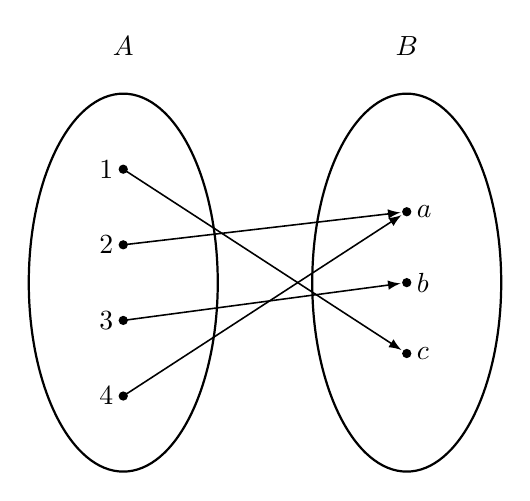
\begin{tikzpicture}[%
    >=latex,
    line width=0.2mm,
    line cap=round,
    scale=1.2
]
    % Coorindates.
    \coordinate (a) at ( 1.5,  0.75);
    \coordinate (b) at ( 1.5, -0.00);
    \coordinate (c) at ( 1.5, -0.75);
    \coordinate (1) at (-1.5,  1.20);
    \coordinate (2) at (-1.5,  0.40);
    \coordinate (3) at (-1.5, -0.40);
    \coordinate (4) at (-1.5, -1.20);
    \coordinate (A) at (-1.5,  2.50);
    \coordinate (B) at ( 1.5,  2.50);

    % Ellipses representing the sets A and B.
    \draw[thick] (-1.5, 0.0) ellipse (1 and 2);
    \draw[thick] ( 1.5, 0.0) ellipse (1 and 2);

    % Draw circles for the various points.
    \draw[fill=black] (a) circle (0.4mm);
    \draw[fill=black] (b) circle (0.4mm);
    \draw[fill=black] (c) circle (0.4mm);
    \draw[fill=black] (1) circle (0.4mm);
    \draw[fill=black] (2) circle (0.4mm);
    \draw[fill=black] (3) circle (0.4mm);
    \draw[fill=black] (4) circle (0.4mm);

    % Draw paths indicating mappings.
    \begin{scope}[->]
        \draw[shorten >=0.8mm] (1) to (c);
        \draw[shorten >=0.8mm] (2) to (a);
        \draw[shorten >=0.8mm] (3) to (b);
        \draw[shorten >=0.8mm] (4) to (a);
    \end{scope}

    % Labels.
    \node at (A)         {$A$};
    \node at (B)         {$B$};
    \node at (a) [right] {$a$};
    \node at (b) [right] {$b$};
    \node at (c) [right] {$c$};
    \node at (1) [left]  {$1$};
    \node at (2) [left]  {$2$};
    \node at (3) [left]  {$3$};
    \node at (4) [left]  {$4$};
\end{tikzpicture}
                }
                \subcaption{A Valid Function.}
            \end{subfigure}
            \begin{subfigure}[b]{0.49\textwidth}
                \centering
                \resizebox{\textwidth}{!}{%
                    %--------------------------------Dependencies----------------------------------%
%   tikz                                                                       %
%       arrows.meta                                                            %
%-------------------------------Main Document----------------------------------%
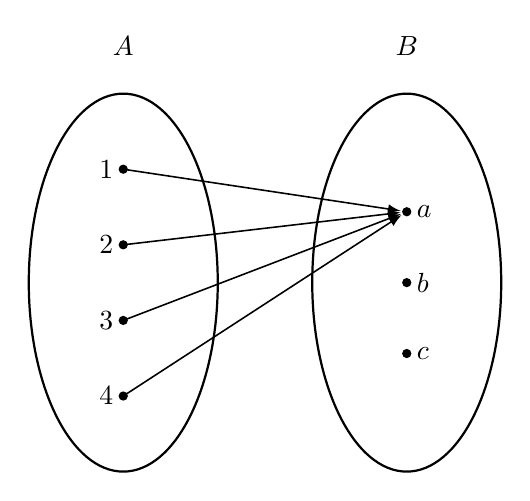
\begin{tikzpicture}[%
    >=latex,
    line width=0.2mm,
    line cap=round,
    scale=1.2
]
    % Coorindates.
    \coordinate (a) at ( 1.5,  0.75);
    \coordinate (b) at ( 1.5, -0.00);
    \coordinate (c) at ( 1.5, -0.75);
    \coordinate (1) at (-1.5,  1.20);
    \coordinate (2) at (-1.5,  0.40);
    \coordinate (3) at (-1.5, -0.40);
    \coordinate (4) at (-1.5, -1.20);
    \coordinate (A) at (-1.5,  2.50);
    \coordinate (B) at ( 1.5,  2.50);

    % Ellipses representing the sets A and B.
    \draw[thick] (-1.5, 0.0) ellipse (1 and 2);
    \draw[thick] ( 1.5, 0.0) ellipse (1 and 2);

    % Draw circles for the various points.
    \draw[fill=black] (a) circle (0.4mm);
    \draw[fill=black] (b) circle (0.4mm);
    \draw[fill=black] (c) circle (0.4mm);
    \draw[fill=black] (1) circle (0.4mm);
    \draw[fill=black] (2) circle (0.4mm);
    \draw[fill=black] (3) circle (0.4mm);
    \draw[fill=black] (4) circle (0.4mm);

    % Draw paths indicating mappings.
    \begin{scope}[->]
        \draw[shorten >=0.8mm] (1) to (a);
        \draw[shorten >=0.8mm] (2) to (a);
        \draw[shorten >=0.8mm] (3) to (a);
        \draw[shorten >=0.8mm] (4) to (a);
    \end{scope}

    % Labels.
    \node at (A)         {$A$};
    \node at (B)         {$B$};
    \node at (a) [right] {$a$};
    \node at (b) [right] {$b$};
    \node at (c) [right] {$c$};
    \node at (1) [left]  {$1$};
    \node at (2) [left]  {$2$};
    \node at (3) [left]  {$3$};
    \node at (4) [left]  {$4$};
\end{tikzpicture}
                }
                \subcaption{Another Valid Function.}
            \end{subfigure}
            \caption{Visual for Abstract Functions}
            \label{fig:Abstract_Functions}
        \end{figure}
        \begin{figure}[H]
            \centering
            \begin{subfigure}[b]{0.49\textwidth}
                \centering
                \resizebox{\textwidth}{!}{%
                    %--------------------------------Dependencies----------------------------------%
%   tikz                                                                       %
%       arrows.meta                                                            %
%-------------------------------Main Document----------------------------------%
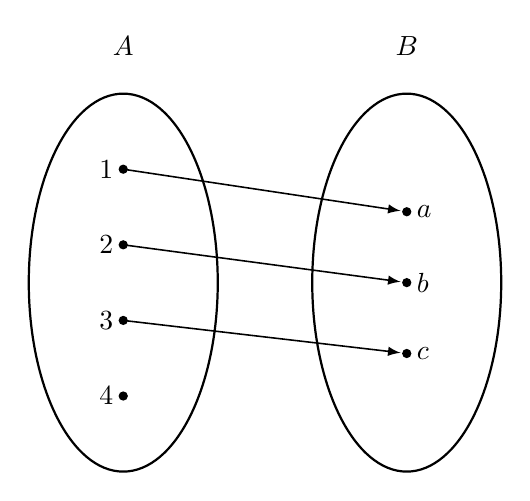
\begin{tikzpicture}[%
    >=latex,
    line width=0.2mm,
    line cap=round,
    scale=1.2
]
    % Coorindates.
    \coordinate (a) at ( 1.5,  0.75);
    \coordinate (b) at ( 1.5, -0.00);
    \coordinate (c) at ( 1.5, -0.75);
    \coordinate (1) at (-1.5,  1.20);
    \coordinate (2) at (-1.5,  0.40);
    \coordinate (3) at (-1.5, -0.40);
    \coordinate (4) at (-1.5, -1.20);
    \coordinate (A) at (-1.5,  2.50);
    \coordinate (B) at ( 1.5,  2.50);

    % Ellipses representing the sets A and B.
    \draw[thick] (-1.5, 0.0) ellipse (1 and 2);
    \draw[thick] ( 1.5, 0.0) ellipse (1 and 2);

    % Draw circles for the various points.
    \draw[fill=black] (a) circle (0.4mm);
    \draw[fill=black] (b) circle (0.4mm);
    \draw[fill=black] (c) circle (0.4mm);
    \draw[fill=black] (1) circle (0.4mm);
    \draw[fill=black] (2) circle (0.4mm);
    \draw[fill=black] (3) circle (0.4mm);
    \draw[fill=black] (4) circle (0.4mm);

    % Draw paths indicating mappings.
    \begin{scope}[->]
        \draw[shorten >=0.8mm] (1) to (a);
        \draw[shorten >=0.8mm] (2) to (b);
        \draw[shorten >=0.8mm] (3) to (c);
    \end{scope}

    % Labels.
    \node at (A)         {$A$};
    \node at (B)         {$B$};
    \node at (a) [right] {$a$};
    \node at (b) [right] {$b$};
    \node at (c) [right] {$c$};
    \node at (1) [left]  {$1$};
    \node at (2) [left]  {$2$};
    \node at (3) [left]  {$3$};
    \node at (4) [left]  {$4$};
\end{tikzpicture}
                }
                \subcaption{Fails Existence.}
            \end{subfigure}
            \begin{subfigure}[b]{0.49\textwidth}
                \centering
                \resizebox{\textwidth}{!}{%
                    %--------------------------------Dependencies----------------------------------%
%   tikz                                                                       %
%       arrows.meta                                                            %
%-------------------------------Main Document----------------------------------%
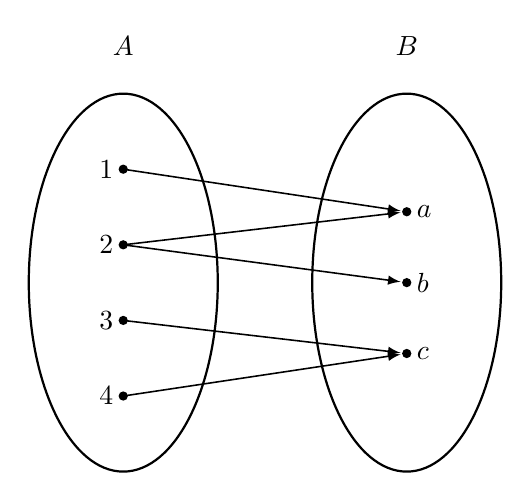
\begin{tikzpicture}[%
    >=latex,
    line width=0.2mm,
    line cap=round,
    scale=1.2
]
    % Coorindates.
    \coordinate (a) at ( 1.5,  0.75);
    \coordinate (b) at ( 1.5, -0.00);
    \coordinate (c) at ( 1.5, -0.75);
    \coordinate (1) at (-1.5,  1.20);
    \coordinate (2) at (-1.5,  0.40);
    \coordinate (3) at (-1.5, -0.40);
    \coordinate (4) at (-1.5, -1.20);
    \coordinate (A) at (-1.5,  2.50);
    \coordinate (B) at ( 1.5,  2.50);

    % Ellipses representing the sets A and B.
    \draw[thick] (-1.5, 0.0) ellipse (1 and 2);
    \draw[thick] ( 1.5, 0.0) ellipse (1 and 2);

    % Draw circles for the various points.
    \draw[fill=black] (a) circle (0.4mm);
    \draw[fill=black] (b) circle (0.4mm);
    \draw[fill=black] (c) circle (0.4mm);
    \draw[fill=black] (1) circle (0.4mm);
    \draw[fill=black] (2) circle (0.4mm);
    \draw[fill=black] (3) circle (0.4mm);
    \draw[fill=black] (4) circle (0.4mm);

    % Draw paths indicating mappings.
    \begin{scope}[->]
        \draw[shorten >=0.8mm] (1) to (a);
        \draw[shorten >=0.8mm] (2) to (a);
        \draw[shorten >=0.8mm] (2) to (b);
        \draw[shorten >=0.8mm] (3) to (c);
        \draw[shorten >=0.8mm] (4) to (c);
    \end{scope}

    % Labels.
    \node at (A)         {$A$};
    \node at (B)         {$B$};
    \node at (a) [right] {$a$};
    \node at (b) [right] {$b$};
    \node at (c) [right] {$c$};
    \node at (1) [left]  {$1$};
    \node at (2) [left]  {$2$};
    \node at (3) [left]  {$3$};
    \node at (4) [left]  {$4$};
\end{tikzpicture}
                }
                \subcaption{Fails Uniqueness.}
            \end{subfigure}
            \caption{Non-Functions}
            \label{fig:Abstract_Non_Functions}
        \end{figure}
        It is possible to count the total number of functions from $A$ to $B$.
        Since every element of $A$ needs to be mapped to some element of $B$,
        and since there are 4 elements in $A$ and 3 elements in $B$, the total
        number of functions $f:A\rightarrow{B}$ is $4^{3}=64$. On the other
        hand, the total number of subsets of $A\times{B}$ is $2^{12}=4096$
        (we will justify this when we discuss the \textit{cardinality} of
        sets). Thus, if we were to randomly pick a subset of $A\times{B}$, the
        odds are that it is almost certainly \textit{not} a function
        (1.5625\%). Thus, functions are very special subsets.
        There is a frequent need to discuss the \textit{set of all functions}
        from a given set $A$ into another set $B$. To ensure we don't create
        a function version of Russell's paradox, we prove such a set exists.
        \begin{theorem}
            If $A$ and $B$ are sets, then there exists a set $\mathcal{F}$ such
            that, for all $f$ it is true that $f\in\mathcal{F}$ if and only if
            $f$ is a function from $A$ to $B$, $f:A\rightarrow{B}$.
            \index{Function!Set of All}
        \end{theorem}
        \begin{proof}
            For if $A$ and $B$ are sets, then by
            Thm.~\ref{thm:Existence_of_the_Cartesian_Product} the set
            $A\times{B}$ exists. But by
            Thm.~\ref{thm:Existence_of_the_Power_Set}, the power set of
            $A\times{B}$, $\mathcal{P}(A\times{B})$, exists. Let $P$ be the
            proposition \textit{True if} $f$ \textit{is a function from} $A$
            \textit{to} $B$, \textit{false otherwise}. Then by axiom schema of
            specification (Ax.~\ref{ax:Axiom_Schema_of_Specification}), there is
            a set $\mathcal{F}$ such that:
            \begin{equation}
                \mathcal{F}=\big\{\,f\in\mathcal{P}(A\times{B})\;|
                    \;P(f)\,\big\}
            \end{equation}
            But then for all $f$, $f\in\mathcal{F}$ if and only if
            $f\in\mathcal{F}$ and $P(f)$ is true. But if $P(f)$ is true then
            $f$ is a function from $A$ to $B$, and thus by the definition of a
            function (Def.~\ref{def:Function}) $f\subseteq{A}\times{B}$. But
            then by the definition of the power set (Def.~\ref{def:Power_Set})
            we have that $f\in\mathcal{P}(A\times{B})$. Thus $P(f)$ implies
            $f\in\mathcal{F}$. Therefore $f\in\mathcal{F}$ if and only if
            $P(f)$. That is, $f\in\mathcal{F}$ if and only if $f$ is a function
            from $A$ to $B$.
        \end{proof}
        There is non-standard notation when discussing the set of all functions
        from a given set $A$ to a set $B$:
        \begin{fnotation}{Set of All Functions}{Set_of_All_Functions}
            If $A$ and $B$ are sets, the set of all functions from $A$ to $B$,
            $f:A\rightarrow{B}$, is denoted as either $\mathcal{F}(A,B)$ or
            $B^{A}$.
        \end{fnotation}
        The notation $B^{A}$ is common in many areas such as topology and
        algebra, especially when $A=B$. The \textit{topological space} $I^{I}$,
        which is the set of all functions from the \textit{closed unit inverval}
        \index{Interval!Closed} to itself, is often used to construct examples
        and counterexamples. In analysis the notation $\mathcal{F}(A,B)$ seems
        to be more common, in particular $\mathcal{C}(A,B)$ is often used to
        denote the set of all \textit{continuous} functions from $A$ to $B$,
        provided the word continuous has meaning. Since the notation is not
        universal nor standard across the various disciplines, an attempt will
        be made to specify what $B^{A}$ or $\mathcal{F}(A,B)$ means before using
        it in a theorem or counterexample.
        \begin{fdefinition}{Image of a Point}{Image_of_Point}
            The \gls{image of a point} of an element $x$ in a set $A$ under a
            \gls{function} $f:A\rightarrow{B}$ is the unique value $y\in{B}$
            such that $(x,y)\in{f}$. We write $y=f(x)$.
            \index{Image!of a Point}
        \end{fdefinition}
        This allows us to define functions by simply specifying what the
        image of each $x\in{A}$ is. Restating our previous claim, if we can
        define some formula such that for each $x\in{A}$ there is a unique
        $f(x)\in{B}$ such that the formula takes $x$ to $f(x)$, then we can
        define $f$ as the set of all such ordered pairs $(x,f(x))$, and this
        will be a function.
        \begin{fnotation}{Image Notation}{Image_Notation}
            If $A$ and $B$ are sets, if $f:A\rightarrow{B}$ is a function,
            if $x\in{A}$ and if $y=f(x)\in{B}$, then we denote this by
            writing $x\overset{f}{\longmapsto}{y}$ or just $x\mapsto{y}$.
        \end{fnotation}
        Throughout we will almost exclusively use the notation $y=f(x)$ rather
        than $x\mapsto{y}$. The reasons are purely aesthetic and both notations
        are common in mathematics. In a similar manner, we can define the image
        of an entire subset.
        \begin{theorem}
            If $A$ and $B$ are sets, if $f:A\rightarrow{B}$ is a function,
            and if $\mathcal{U}\subseteq{A}$, then there is a set
            $\mathcal{V}\subseteq{B}$ such that for all $y$ it is true that
            $y\in\mathcal{V}$ if and only if $y\in{B}$ and such that there is
            an $x\in\mathcal{U}$ such that $y=f(x)$.
        \end{theorem}
        \begin{proof}
            For let $P$ be the proposition \textit{True if there exists}
            $x\in\mathcal{U}$ \textit{such that} $y=f(x)$,
            \textit{false otherwise}. By the axiom schema of specification
            (Ax.~\ref{ax:Axiom_Schema_of_Specification}) there is a set
            $\mathcal{V}$ such that, for all $y$ it is true that
            $y\in\mathcal{V}$ if and only if $y\in{B}$ and $P(y)$ is true. That
            is, $y\in\mathcal{V}$ if and only if $y\in{B}$ and if there is an
            $x\in\mathcal{U}$ such that $y=f(x)$.
        \end{proof}
        \begin{fdefinition}{Image of a Subset}{Image_of_Subset}
            The \gls{set image} of a \gls{subset} $\mathcal{U}$ of a \gls{set}
            $A$ under a \gls{function} $f:A\rightarrow{B}$ is the
            set:\index{Image!of a Set}
            \begin{equation*}
                f\big(\mathcal{U}\big)=
                    \{\,y\in{B}\;|\;\textrm{There exists }x\in\mathcal{U}
                                    \textrm{ such that }y=f(x)\,\}
            \end{equation*}
            That is, the set of all points in $B$ that are the image of points
            in $\mathcal{U}$. Formally:
            \begin{equation*}
                \forall_{A}\forall_{B}\forall_{f:A\rightarrow{B}}
                \forall_{\mathcal{U}\subseteq{A}}\forall_{y}\Big(
                    \big(y\in{f}(\mathcal{U})\big)\Longleftrightarrow
                    \big(\exists_{x\in\mathcal{U}}:y=f(x)\big)\Big)
            \end{equation*}
        \end{fdefinition}
        This definition of the image of a subset was given in such a manner
        so that it only relies on the axiom schema of specification to
        justify it's existence. We could also use the notation:
        \begin{equation}
            f\big(\mathcal{U})=\{\,f(x)\in{B}\;|\;x\in\mathcal{U}\,\}
        \end{equation}
        Writing the definition of the image of a subset in such a way is
        justified by the \textit{axiom schema of replacement}%
        \index{Axiom!Schema of Replacement}, but we've not yet included this
        axiom in our system.
        \begin{example}
            If $f:\mathbb{R}\rightarrow\mathbb{R}$ is the function $f(x)=x^{2}$,
            then:
            \begin{equation}
                f(\mathbb{R})=[0,\infty)\equiv\{\,x\in\mathbb{R}\;|\;x\geq{0}\}
            \end{equation}
            This is because every non-negative real number $y$ gets mapped to
            by at least one real number (the positive square root $\sqrt{y}$).
            None of the negative numbers are the image of any element of
            $\mathbb{R}$ since the square of a real number is always
            non-negative.
        \end{example}
        We can visualize functions and images by using blobs in the plane. Given
        some sub-blob of a set $A$, the image of this will be another sub-blob
        of $B$. Note that if $f:A\rightarrow{B}$ is a function, it does
        \textbf{not} need to be true that $f(A)=B$. These are special functions
        that are called \textit{surjective}\index{Function!Surjective} and are
        discussed in Chapt.~\ref{chapt:Function_Theory}. Such a drawing of the
        general case is shown in Fig.~\ref{fig:Image_of_Point_and_Subset}.
        \begin{figure}[H]
            \centering
            \captionsetup{type=figure}
            \begin{tikzpicture}[>=Latex]
    \coordinate (U1) at (-5.0, -2.0);
    \coordinate (U2) at (-3.5, -2.0);
    \coordinate (U3) at (-0.5, -0.5);
    \coordinate (U4) at (-2.0,  2.0);
    \coordinate (U5) at (-3.3,  1.6);
    \coordinate (U6) at (-4.0,  2.0);
    \coordinate (U7) at (-5.0,  0.0);

    \coordinate (V1) at (5.0,  2.0);
    \coordinate (V2) at (4.0,  2.0);
    \coordinate (V3) at (2.0,  0.0);
    \coordinate (V4) at (2.0, -2.0);
    \coordinate (V5) at (4.0, -1.0);
    \coordinate (V6) at (5.0, -1.0);

    \coordinate (S1) at (-4.0,  0.0);
    \coordinate (S2) at (-3.0, -1.0);
    \coordinate (S3) at (-2.5,  0.0);
    \coordinate (S4) at (-3.0,  0.5);

    \coordinate (T1) at (3.0,  0.0);
    \coordinate (T2) at (3.5, -0.8);
    \coordinate (T3) at (4.5,  0.0);
    \coordinate (T4) at (3.5,  0.8);

    \coordinate (x)  at (-2.8, -0.3);
    \coordinate (fx) at (3.4,  -0.4);

    \draw[fill=blue,opacity=0.5,draw=black,thick]
        (U1)    to[out=0,  in=-150] (U2)
                to[out=30, in=-90]  (U3)
                to[out=90, in=-60]  (U4)
                to[out=120, in=-30] (U5)
                to[out=150,in=10]   (U6)
                to[out=-170,in=90]  (U7)
                to[out=-90,in=180]  cycle;

    \draw[fill=red!80!white,opacity=0.5,draw=black,thick]
        (V1)    to[out=180, in=0]       (V2)
                to[out=180, in=60]      (V3)
                to[out=-120,in=120]     (V4)
                to[out=-60, in=180]     (V5)
                to[out=0,   in=-120]    (V6)
                to[out=60,  in=0]       cycle;

    \draw[fill=blue!80!white] (S1)  to[out=-150,in=180] (S2)
                                    to[out=0,   in=-90] (S3)
                                    to[out=90,  in=-60] (S4)
                                    to[out=120, in=30]  cycle;

    \draw[fill=red!80!white] (T1)   to[out=-150,in=180] (T2)
                                    to[out=0,   in=-90] (T3)
                                    to[out=90,  in=0]   (T4)
                                    to[out=180, in=30]  cycle;

    \draw[fill=black] (x)  circle (0.3mm);
    \draw[fill=black] (fx) circle (0.3mm);
    \node at (-2.5, 1.0) {\Large{$A$}};
    \node at ( 4.6, 1.3) {\Large{$B$}};
    \node at (-3.3, 0.0) {\large{$\mathcal{U}$}};
    \node at ( 3.7, 0.2) {\large{$f(\mathcal{U})$}};
    \node at (x)  [below] {$x$};
    \node at (fx) [right] {$f(x)$};
    \draw[->,shorten >= 1.5mm,shorten <= 1.5mm]
        (x) to[out=-30,in=-150] node[below]{$f$} (fx);
\end{tikzpicture}
            \caption{Image of a Subset and of a Point under a Function}
            \label{fig:Image_of_Point_and_Subset}
        \end{figure}
        If we consider a function $f:A\rightarrow{B}$ and the image of the
        entire set $A$ we obtain the \textit{range} of $f$. That is, the range
        is the set $f(A)\subseteq{B}$. In a similar manner to the forward image
        of a function, we can define the pre-image.
        \begin{theorem}
            \label{thm:Existence_of_Pre_Image}%
            If $A$ and $B$ are sets, if $f:A\rightarrow{B}$ is a function from
            $A$ to $B$, and if $\mathcal{V}\subseteq{B}$, then there is a set
            $\mathcal{U}\subseteq{A}$ such that for all $x$ it is true that
            $x\in\mathcal{U}$ if and only if $x\in{A}$ and $f(x)\in\mathcal{V}$.
        \end{theorem}
        \begin{proof}
            For let $P$ be the proposition \textit{True if} $x\in{A}$
            \textit{and} $f(x)\in\mathcal{V}$, \textit{false otherwise}. Then
            by the axiom schema of specification
            (Ax.~\ref{ax:Axiom_Schema_of_Specification}) there is a set
            $\mathcal{U}$ such that:
            \begin{equation*}
                \mathcal{U}=\big\{\,x\in{A}\;|\;P(x)\,\big\}
            \end{equation*}
            But $P(x)$ implies $x\in{A}$ and thus $x\in\mathcal{U}$ if and only
            if $x\in{A}$ and $f(x)\in\mathcal{V}$.
        \end{proof}
        \begin{fdefinition}{Pre-Image of a Subset}{Pre_Image_of_Subset}
            The \gls{pre-image} of a \gls{subset} $\mathcal{V}\subseteq{B}$
            under a \gls{function} $f:A\rightarrow{B}$ is the set:
            \index{Pre-Image}
            \begin{equation}
                f^{\minus{1}}(\mathcal{V})
                =\big\{\,x\in{A}\;|\;f(x)\in\mathcal{V}\,\big\}
            \end{equation}
            Using our formal language:
            \begin{equation*}
                \forall_{A}\forall_{B}\forall_{f:A\rightarrow{B}}
                \forall_{\mathcal{V}\subseteq{B}}\forall_{x}\Big(
                    \big(x\in{f}^{\minus{1}}(\mathcal{V})\big)
                    \Longleftrightarrow
                    \big((x\in{A})\land(f(x)\in\mathcal{V}))\big)\Big)
            \end{equation*}
        \end{fdefinition}
        The pre-image of a set behaves a lot differently than the image, and
        this will be explored in detail when functions are discussed. The cause
        of the discrepancy is the requirement that elements of $A$ map uniquely
        to elements of $B$, but a single element in $B$ can be the image of
        many different points in $A$. This gives rise to the notion of the
        \textit{fiber} of a point in $B$.
        \begin{theorem}
            If $A$ and $B$ are sets, if $f:A\rightarrow{B}$ is a function, and
            if $b\in{A}$, then there is a set $\mathcal{U}\subseteq{A}$ such
            for all $x\in{A}$ it is true that $x\in\mathcal{U}$ if and only if
            $f(x)=b$.
        \end{theorem}
        \begin{proof}
            For by Thm.~\ref{thm:Existence_of_Set_Containing_Set}, $\{b\}$ is
            a set and $\{b\}\subseteq{B}$ (Def.~\ref{def:Subsets}). But if
            $\{b\}$ is a subset of $B$, then there is a set
            $\mathcal{U}\subseteq{A}$ such that for all $x\in{A}$ it is true
            that $x\in\mathcal{U}$ if and only if $f(x)\in\{b\}$
            (Thm.~\ref{thm:Existence_of_Pre_Image}). But $f(x)\in\{b\}$ if and
            only if $f(x)=b$ (Thm.~\ref{thm:Existence_of_Set_Containing_Set}).
            Thus, for all $x\in{A}$, $x\in\mathcal{U}$ if and only if $f(x)=b$.
        \end{proof}
        \begin{fdefinition}{Fiber of an Element}{Fiber_of_Element}
            The \gls{fiber} of an element $b$ in a \gls{set} $B$ under a
            \gls{function} $f:A\rightarrow{B}$ from a set $A$ to a set $B$ is
            the pre-image of the set $\{b\}$. That is:\index{Fiber}
            \begin{equation*}
                f^{\minus{1}}(\{b\})
                =\big\{\,a\in{A}\:|\;f(a)=b\,\big\}
            \end{equation*}
        \end{fdefinition}
        Before we end our introduction to the concept of a function, we should
        first note the other synonomous terminology that is used and give some
        historical background. In many texts, including this one, authors use
        the word \textit{map} or \textit{mapping} to denote a function, rather
        than simply use the word function. This language has its roots in
        geometry, and particularly in the study of projective geometry. One can
        consider \textit{perspectives}, which are functions that map one line in
        the Euclidean plane to another. Consider two non-parallel lines
        $\overline{AB}$ and $\overline{CD}$ and a point $P$ in the plane that
        lies on neither of these two. Given a point $x$ which lies on
        $\overline{AB}$, we map this to the line $\overline{CD}$ by drawing a
        straight line from $P$ to $x$ and marking where this intersects
        $\overline{CD}$
        (see Fig.~\ref{fig:Example_of_Map_from_Projective_Geometry}).
        \begin{figure}[H]
            \centering
            \captionsetup{type=figure}
            \includegraphics{images/perspective_lines_001.pdf}
            \caption{Example of a Mapping from Projective Geometry}
            \label{fig:Example_of_Map_from_Projective_Geometry}
        \end{figure}
        Such constructions play a central role in geometry, and particularly
        projective geometry, and culminate in a beautiful theorem known as
        \textit{Desargues's Theorem}\index{Theorem!Desargues's}, named after
        Girard Desargues. From this historical motivation, the word function,
        map, and mapping are synonomous in the realm of mathematics. In select
        fields such as analysis and geometry the words \textit{operator} and
        \textit{transformation} are used, and occasionally the word
        \textit{graph} is used. We will try to be clear in our useage of this
        vocabularly to rid of any potential ambiguity.
    \subsection{The Axiom of Choice and Diaconescu's Theorem}
        The next two axioms to be introduced are the most controversial of those
        listed in ZFC: The \textit{axiom of infinity} and the
        \textit{axiom of choice}. While the axiom of infinity only has a
        small number of critics, the axiom of choice is far more contentious.
        Choice is equivalent to many other statements that come across in
        almost all forms of mathematics (analysis, algebra, topology, etc.).
        Many of which are theorems we would \textit{want} to be true, and so
        accepting the axiom of choice allows us to prove them. In particular,
        the axioms presented thus far can be combined with the axiom of choice
        to prove the \textit{Law of the Excluded Middle}, a result known as
        Diaconescu's theorem, and this is our current goal.
        \begin{faxiom}{Axiom of Choice}{Axiom_of_Choice}
            If $\mathcal{O}$ is a non-empty set such that for all
            $\mathcal{U}\in\mathcal{O}$ it is true that $\mathcal{U}$ is
            non-empty, and if $\bigcup\mathcal{O}$ is the union over
            $\mathcal{O}$, then there is a function
            $f:\mathcal{O}\rightarrow\mathcal{F}$ such that for all
            $x\in\mathcal{O}$ it is true that $f(x)\in{x}$.
            Formally:\index{Axiom!of Choice}
            \begin{equation*}
                \forall_{\mathcal{O}}\big((\mathcal{O}\ne\emptyset)\land
                    (\emptyset\notin\mathcal{O})\big)
                \exists_{f:\mathcal{O}\rightarrow\bigcup\mathcal{O}}\Big(
                \forall_{x\in\mathcal{O}}\big(f(x)\in{x}\big)\Big)
            \end{equation*}
        \end{faxiom}
        Such a function is called a \textit{choice function}%
        \index{Function!Choice Function}. The axiom can be made obviously true
        or obviously false depending on how we word it. To convince one of its
        validity requires talking about products\index{Product!of Sets}. The
        Cartesian product\index{Cartesian Product} has been defined using
        ordered pairs\index{Ordered Pair} as defined by
        Kuratowski\index{Kuratowski, Kazimierz} and allows us to order two
        elements. Given two sets $A$ and $B$ we can define an equivalent notion
        using the set of all functions from $\mathbb{Z}_{2}=\{0,1\}$ into
        $A\cup{B}$ with a particular property:
        \begin{equation}
            A\times{B}=
            \big\{\,f:\mathbb{Z}_{2}\rightarrow{A}\cup{B}\;|\;
                f(0)\in{A}\textrm{ and }f(1)\in{B}\,\big\}
        \end{equation}
        To see why this is equivalent note that $A\times{B}$ is the set of all
        ordered pairs whose first entry lies in $A$ and whose second entry lies
        in $B$. Given $a\in{A}$ and $b\in{B}$, let
        $f:\mathbb{Z}_{2}\rightarrow{A}\cup{B}$ be the function such that
        $f(0)=a$ and $f(1)=b$. Then we can identify the ordered pair $(a,b)$
        with $f$. Indeed, $(a,b)=(f(0),f(1))$ making our identification very
        explicit. We can now generalize to a collection of $n$ different sets
        and define the ordered $n$ tuple over a collection of $n$ sets to be the
        set of all functions from $\mathbb{Z}_{n}$ into the union over this
        collection with a similar property:
        \begin{equation}
            \prod_{k\in\mathbb{Z}_{n}}A_{k}
            =\Big\{\,f:\mathbb{Z}_{n}\rightarrow\bigcup_{k\in\mathbb{Z}_{n}}^{n}
                A_{k}\;\big|\;f(k)\in{A}_{k}\textrm{ for all }k\in\mathbb{Z}_{n}
            \Big\}
        \end{equation}
        Given the function $f$ that maps $k$ to $a_{k}\in{A}_{k}$, we identify
        this by:
        \begin{equation}
            f=(a_{0},\,a_{1},\,\dots,\,a_{k},\,\dots,\,a_{n-1})
            =(f(0),\,f(1),\,\dots,\,f(k),\,\dots,\,f(n-1))
        \end{equation}
        And thus we have a more general way of defining products. Note that
        swapping the order of the product is equivalent to changing functions,
        so two $n$ tuples are equal if and only if all of their entries are
        equal. What's nice about our function definition is that it allows one
        to define products over \textit{arbitrary} collections. This is crucial
        for topology and analysis as we often wish to speak of
        \textit{infinite dimensional} spaces that are constructed using these
        abstract products. Given a set $I$, often called the \textit{index set},
        such that for all $\mathcal{U}\in{I}$ it is true $\mathcal{U}$ is a set,
        we can form the product over $I$ by defining this to be the collection
        of all functions from $I$ into the union over $I$.
        \begin{equation}
            \prod_{i\in{I}}A_{i}
            =\big\{\,f:I\rightarrow\bigcup_{i\in{I}}A_{i}\;|\;
                f(i)\in{A}_{i}\textrm{ for all }i\in{I}\,\big\}
        \end{equation}
        The axiom of choice\index{Axiom!of Choice} is equivalent to the
        statement \textit{The infinite product of non-empty sets is non-empty}.
        These functions that identify $k$ with the $k^{th}$ set are precisely
        choice functions. Phrasing it like this we see that the axiom of choice
        is somewhat obvious. The infinite product of non-empty sets is most
        likely enormous! Claiming it's non-empty seems trivial. It is then
        unfortunate that this claim can not be proven with the other axioms
        we've developed. As stated before, the axiom of choice is equivalent to
        many other statements such as \textit{Zorn's lemma, Tychonoff's theorem,
        the well ordering theorem, every vector space has a basis, every set has
        a group structure}, and countless more. Many of these theorems have many
        applications to algebra, analysis, and topology, and since we would like
        to use them to prove other things we are forced to accept the axiom of
        choice. Many theorems in real analysis hide the use of the axiom of
        choice by constructing sequences \textit{by induction}. An attempt will
        be made to be clear whenever the axiom of choice is used in a proof.
        \par\hfill\par
        We conclude this section by presenting Diaconescu's theorem.
        \begin{ftheorem}{Diaconescu's Theorem}{Diaconescus_Theorem}
            If $P$ is a proposition on sets and if $x$ is a set, then either
            $P(x)$ is true or the negation of $P(x)$ is true. That is,
            $P\lor\neg{P}$ is true.
            \index{Theorem!Diaconescu's}
        \end{ftheorem}
        \begin{bproof}
            Let $0=\emptyset$. By
            Thm.~\ref{thm:Existence_of_Set_Containing_Set}, we have that the set
            $\{0\}$ exists. Let $1=\{0\}$. Then since $0\in{1}$, $0\ne{1}$
            (Thm.~\ref{thm:Containment_NEqual_Underlying_Set}). Since $0$ and
            $1$ are sets, by Thm.~\ref{thm:Existence_of_Set_Built_from_Two_Sets}
            we have that the set $\{0,1\}$ exists. Let $Q$ be the proposition
            \textit{true if P(x) or } $x=0$, \textit{false otherwise}. By the
            axiom schema of specification
            (Ax.~\ref{ax:Axiom_Schema_of_Specification}) there exists a set
            $\mathcal{U}$ such that:
            \begin{equation}
                \mathcal{U}=\big\{\,x\in\{\,0,\,1\,\}\;|\;Q(x)\,\big\}
            \end{equation}
            Similarly, let $R$ be the proposition \textit{true if P(x) or}
            $x=1$, \textit{false otherwise}. By the axiom schema of
            specification we have that the following set exists:
            \begin{equation}
                \mathcal{V}=\big\{\,x\in\{\,0,\,1\,\}\;|\;R(x)\,\big\}
            \end{equation}
            By Thm.~\ref{thm:Existence_of_Set_Built_from_Two_Sets}, we have that
            the set $\{\,\mathcal{U},\,\mathcal{V}\,\}$ exists. By the axiom of
            choice (Ax.~\ref{ax:Axiom_of_Choice}), there exists a function
            $f:\{\mathcal{U},\mathcal{V}\}\rightarrow%
             \bigcup\{\mathcal{U},\mathcal{V}\}$ such that
            $f(\mathcal{U})\in\mathcal{U}$ and $f(\mathcal{V})\in\mathcal{V}$.
            But then, by the definition of $\mathcal{U}$, either
            $f(\mathcal{U})=0$ or $P(x)$ is true. Similarly, either
            $f(\mathcal{V})=1$ or $P(x)$ is true. But since $0\ne{1}$, either
            $f(\mathcal{U})\ne{f}(\mathcal{V})$ or $P(x)$ is true. Again by the
            axiom of extensionality (Ax.~\ref{ax:Axiom_of_Extensionality}), and
            by the definition of $\mathcal{U}$ and $\mathcal{V}$, if $P(x)$ is
            true then $\mathcal{U}=\mathcal{V}$. But then
            $f(\mathcal{U})=f(\mathcal{V})$. But then, by the contrapositive,
            $\neg{P}(x)$ implies that $f(\mathcal{U})\ne{f}(\mathcal{V})$. But
            by extensionality, either $f(\mathcal{U})=f(\mathcal{V})$ or
            $f(\mathcal{U})\ne{f}(\mathcal{V})$, and thus either $P(x)$ or
            $\neg{P}(x)$. That is, $P\lor\neg{P}$ is true.
        \end{bproof}
        We can now prove things via \textit{proof by contradiction}. While we
        have made great efforts to justify every step of a proof thus far, we
        will often omit mention of Diaconescu's theorem as a justification for
        the law of the excluded middle and simply use it freely. We may rest
        easy knowing that we've proved it's validity within the framework of
        ZFC. There are two more axioms remaining, that of infinity and
        replacement. The axiom of infinity is best introduced when we construct
        the natural numbers, and from there build the real numbers, and thus we
        shall delay its development briefly. The axiom of replacement needs a
        notion of class and thus will also be postponed.
